
%% bare_conf.tex
%% V1.3
%% 2007/01/11
%% by Michael Shell
%% See:
%% http://www.michaelshell.org/
%% for current contact information.
%%
%% This is a skeleton file demonstrating the use of IEEEtran.cls
%% (requires IEEEtran.cls version 1.7 or later) with an IEEE conference paper.
%%
%% Support sites:
%% http://www.michaelshell.org/tex/ieeetran/
%% http://www.ctan.org/tex-archive/macros/latex/contrib/IEEEtran/
%% and
%% http://www.ieee.org/

%%*************************************************************************
%% Legal Notice:
%% This code is offered as-is without any warranty either expressed or
%% implied; without even the implied warranty of MERCHANTABILITY or
%% FITNESS FOR A PARTICULAR PURPOSE! 
%% User assumes all risk.
%% In no event shall IEEE or any contributor to this code be liable for
%% any damages or losses, including, but not limited to, incidental,
%% consequential, or any other damages, resulting from the use or misuse
%% of any information contained here.
%%
%% All comments are the opinions of their respective authors and are not
%% necessarily endorsed by the IEEE.
%%
%% This work is distributed under the LaTeX Project Public License (LPPL)
%% ( http://www.latex-project.org/ ) version 1.3, and may be freely used,
%% distributed and modified. A copy of the LPPL, version 1.3, is included
%% in the base LaTeX documentation of all distributions of LaTeX released
%% 2003/12/01 or later.
%% Retain all contribution notices and credits.
%% ** Modified files should be clearly indicated as such, including  **
%% ** renaming them and changing author support contact information. **
%%
%% File list of work: IEEEtran.cls, IEEEtran_HOWTO.pdf, bare_adv.tex,
%%                    bare_conf.tex, bare_jrnl.tex, bare_jrnl_compsoc.tex
%%*************************************************************************

% *** Authors should verify (and, if needed, correct) their LaTeX system  ***
% *** with the testflow diagnostic prior to trusting their LaTeX platform ***
% *** with production work. IEEE's font choices can trigger bugs that do  ***
% *** not appear when using other class files.                            ***
% The testflow support page is at:
% http://www.michaelshell.org/tex/testflow/



% Note that the a4paper option is mainly intended so that authors in
% countries using A4 can easily print to A4 and see how their papers will
% look in print - the typesetting of the document will not typically be
% affected with changes in paper size (but the bottom and side margins will).
% Use the testflow package mentioned above to verify correct handling of
% both paper sizes by the user's LaTeX system.
%
% Also note that the "draftcls" or "draftclsnofoot", not "draft", option
% should be used if it is desired that the figures are to be displayed in
% draft mode.
%
\documentclass[conference]{IEEEtran}
\usepackage{blindtext, graphicx, hyperref, color, caption}
\usepackage[table,xcdraw]{xcolor}
\usepackage{tikz}
\usepackage{mathtools}
\usepackage{pgfplots}
\usepackage{amsmath}
\usepackage{amsfonts}
\usepackage{amssymb}
\usepackage{multicol}
\usepackage{algorithm}
\usepackage{algpseudocode}
\usepackage{amsthm}
\usepackage{amsmath}
\usepackage{fancyhdr}
\usepackage{lastpage}
\usepackage{hhline}
\usetikzlibrary{calc,chains,arrows,shapes,arrows,backgrounds,positioning}

\newtheorem{definition}{Definition}
\newtheorem{example}{Example}[definition]
\newtheorem{theorem}{Theorem}
\newtheorem{corollary}{Corollary}[theorem]
\newtheorem{lemma}[theorem]{Lemma}

\DeclarePairedDelimiter\abs{\lvert}{\rvert}%

\tikzset{
block/.style={
  rectangle,
  draw,
  text width=4.5em,
  text centered,
  rounded corners,
  minimum height=3em},
line/.style={draw, -latex'},
edge/.style={draw},
webservice/.style={
  cloud,
  draw,
  cloud puffs=10,
  cloud puff arc = 120,
  aspect = 2,
  inner ysep =.5em}
}

% Add the compsoc option for Computer Society conferences.
%
% If IEEEtran.cls has not been installed into the LaTeX system files,
% manually specify the path to it like:
% \documentclass[conference]{../sty/IEEEtran}





% Some very useful LaTeX packages include:
% (uncomment the ones you want to load)


% *** MISC UTILITY PACKAGES ***
%
%\usepackage{ifpdf}
% Heiko Oberdiek's ifpdf.sty is very useful if you need conditional
% compilation based on whether the output is pdf or dvi.
% usage:
% \ifpdf
%   % pdf code
% \else
%   % dvi code
% \fi
% The latest version of ifpdf.sty can be obtained from:
% http://www.ctan.org/tex-archive/macros/latex/contrib/oberdiek/
% Also, note that IEEEtran.cls V1.7 and later provides a builtin
% \ifCLASSINFOpdf conditional that works the same way.
% When switching from latex to pdflatex and vice-versa, the compiler may
% have to be run twice to clear warning/error messages.






% *** CITATION PACKAGES ***
%
%\usepackage{cite}
% cite.sty was written by Donald Arseneau
% V1.6 and later of IEEEtran pre-defines the format of the cite.sty package
% \cite{} output to follow that of IEEE. Loading the cite package will
% result in citation numbers being automatically sorted and properly
% "compressed/ranged". e.g., [1], [9], [2], [7], [5], [6] without using
% cite.sty will become [1], [2], [5]--[7], [9] using cite.sty. cite.sty's
% \cite will automatically add leading space, if needed. Use cite.sty's
% noadjust option (cite.sty V3.8 and later) if you want to turn this off.
% cite.sty is already installed on most LaTeX systems. Be sure and use
% version 4.0 (2003-05-27) and later if using hyperref.sty. cite.sty does
% not currently provide for hyperlinked citations.
% The latest version can be obtained at:
% http://www.ctan.org/tex-archive/macros/latex/contrib/cite/
% The documentation is contained in the cite.sty file itself.






% *** GRAPHICS RELATED PACKAGES ***
%
\ifCLASSINFOpdf
  % \usepackage[pdftex]{graphicx}
  % declare the path(s) where your graphic files are
  % \graphicspath{{../pdf/}{../jpeg/}}
  % and their extensions so you won't have to specify these with
  % every instance of \includegraphics
  % \DeclareGraphicsExtensions{.pdf,.jpeg,.png}
\else
  % or other class option (dvipsone, dvipdf, if not using dvips). graphicx
  % will default to the driver specified in the system graphics.cfg if no
  % driver is specified.
  % \usepackage[dvips]{graphicx}
  % declare the path(s) where your graphic files are
  % \graphicspath{{../eps/}}
  % and their extensions so you won't have to specify these with
  % every instance of \includegraphics
  % \DeclareGraphicsExtensions{.eps}
\fi
% graphicx was written by David Carlisle and Sebastian Rahtz. It is
% required if you want graphics, photos, etc. graphicx.sty is already
% installed on most LaTeX systems. The latest version and documentation can
% be obtained at: 
% http://www.ctan.org/tex-archive/macros/latex/required/graphics/
% Another good source of documentation is "Using Imported Graphics in
% LaTeX2e" by Keith Reckdahl which can be found as epslatex.ps or
% epslatex.pdf at: http://www.ctan.org/tex-archive/info/
%
% latex, and pdflatex in dvi mode, support graphics in encapsulated
% postscript (.eps) format. pdflatex in pdf mode supports graphics
% in .pdf, .jpeg, .png and .mps (metapost) formats. Users should ensure
% that all non-photo figures use a vector format (.eps, .pdf, .mps) and
% not a bitmapped formats (.jpeg, .png). IEEE frowns on bitmapped formats
% which can result in "jaggedy"/blurry rendering of lines and letters as
% well as large increases in file sizes.
%
% You can find documentation about the pdfTeX application at:
% http://www.tug.org/applications/pdftex





% *** MATH PACKAGES ***
%
%\usepackage[cmex10]{amsmath}
% A popular package from the American Mathematical Society that provides
% many useful and powerful commands for dealing with mathematics. If using
% it, be sure to load this package with the cmex10 option to ensure that
% only type 1 fonts will utilized at all point sizes. Without this option,
% it is possible that some math symbols, particularly those within
% footnotes, will be rendered in bitmap form which will result in a
% document that can not be IEEE Xplore compliant!
%
% Also, note that the amsmath package sets \interdisplaylinepenalty to 10000
% thus preventing page breaks from occurring within multiline equations. Use:
%\interdisplaylinepenalty=2500
% after loading amsmath to restore such page breaks as IEEEtran.cls normally
% does. amsmath.sty is already installed on most LaTeX systems. The latest
% version and documentation can be obtained at:
% http://www.ctan.org/tex-archive/macros/latex/required/amslatex/math/





% *** SPECIALIZED LIST PACKAGES ***
%
%\usepackage{algorithmic}
% algorithmic.sty was written by Peter Williams and Rogerio Brito.
% This package provides an algorithmic environment fo describing algorithms.
% You can use the algorithmic environment in-text or within a figure
% environment to provide for a floating algorithm. Do NOT use the algorithm
% floating environment provided by algorithm.sty (by the same authors) or
% algorithm2e.sty (by Christophe Fiorio) as IEEE does not use dedicated
% algorithm float types and packages that provide these will not provide
% correct IEEE style captions. The latest version and documentation of
% algorithmic.sty can be obtained at:
% http://www.ctan.org/tex-archive/macros/latex/contrib/algorithms/
% There is also a support site at:
% http://algorithms.berlios.de/index.html
% Also of interest may be the (relatively newer and more customizable)
% algorithmicx.sty package by Szasz Janos:
% http://www.ctan.org/tex-archive/macros/latex/contrib/algorithmicx/




% *** ALIGNMENT PACKAGES ***
%
%\usepackage{array}
% Frank Mittelbach's and David Carlisle's array.sty patches and improves
% the standard LaTeX2e array and tabular environments to provide better
% appearance and additional user controls. As the default LaTeX2e table
% generation code is lacking to the point of almost being broken with
% respect to the quality of the end results, all users are strongly
% advised to use an enhanced (at the very least that provided by array.sty)
% set of table tools. array.sty is already installed on most systems. The
% latest version and documentation can be obtained at:
% http://www.ctan.org/tex-archive/macros/latex/required/tools/


%\usepackage{mdwmath}
%\usepackage{mdwtab}
% Also highly recommended is Mark Wooding's extremely powerful MDW tools,
% especially mdwmath.sty and mdwtab.sty which are used to format equations
% and tables, respectively. The MDWtools set is already installed on most
% LaTeX systems. The lastest version and documentation is available at:
% http://www.ctan.org/tex-archive/macros/latex/contrib/mdwtools/


% IEEEtran contains the IEEEeqnarray family of commands that can be used to
% generate multiline equations as well as matrices, tables, etc., of high
% quality.


%\usepackage{eqparbox}
% Also of notable interest is Scott Pakin's eqparbox package for creating
% (automatically sized) equal width boxes - aka "natural width parboxes".
% Available at:
% http://www.ctan.org/tex-archive/macros/latex/contrib/eqparbox/





% *** SUBFIGURE PACKAGES ***
%\usepackage[tight,footnotesize]{subfigure}
% subfigure.sty was written by Steven Douglas Cochran. This package makes it
% easy to put subfigures in your figures. e.g., "Figure 1a and 1b". For IEEE
% work, it is a good idea to load it with the tight package option to reduce
% the amount of white space around the subfigures. subfigure.sty is already
% installed on most LaTeX systems. The latest version and documentation can
% be obtained at:
% http://www.ctan.org/tex-archive/obsolete/macros/latex/contrib/subfigure/
% subfigure.sty has been superceeded by subfig.sty.



%\usepackage[caption=false]{caption}
%\usepackage[font=footnotesize]{subfig}
% subfig.sty, also written by Steven Douglas Cochran, is the modern
% replacement for subfigure.sty. However, subfig.sty requires and
% automatically loads Axel Sommerfeldt's caption.sty which will override
% IEEEtran.cls handling of captions and this will result in nonIEEE style
% figure/table captions. To prevent this problem, be sure and preload
% caption.sty with its "caption=false" package option. This is will preserve
% IEEEtran.cls handing of captions. Version 1.3 (2005/06/28) and later 
% (recommended due to many improvements over 1.2) of subfig.sty supports
% the caption=false option directly:
%\usepackage[caption=false,font=footnotesize]{subfig}
%
% The latest version and documentation can be obtained at:
% http://www.ctan.org/tex-archive/macros/latex/contrib/subfig/
% The latest version and documentation of caption.sty can be obtained at:
% http://www.ctan.org/tex-archive/macros/latex/contrib/caption/




% *** FLOAT PACKAGES ***
%
%\usepackage{fixltx2e}
% fixltx2e, the successor to the earlier fix2col.sty, was written by
% Frank Mittelbach and David Carlisle. This package corrects a few problems
% in the LaTeX2e kernel, the most notable of which is that in current
% LaTeX2e releases, the ordering of single and double column floats is not
% guaranteed to be preserved. Thus, an unpatched LaTeX2e can allow a
% single column figure to be placed prior to an earlier double column
% figure. The latest version and documentation can be found at:
% http://www.ctan.org/tex-archive/macros/latex/base/



%\usepackage{stfloats}
% stfloats.sty was written by Sigitas Tolusis. This package gives LaTeX2e
% the ability to do double column floats at the bottom of the page as well
% as the top. (e.g., "\begin{figure*}[!b]" is not normally possible in
% LaTeX2e). It also provides a command:
%\fnbelowfloat
% to enable the placement of footnotes below bottom floats (the standard
% LaTeX2e kernel puts them above bottom floats). This is an invasive package
% which rewrites many portions of the LaTeX2e float routines. It may not work
% with other packages that modify the LaTeX2e float routines. The latest
% version and documentation can be obtained at:
% http://www.ctan.org/tex-archive/macros/latex/contrib/sttools/
% Documentation is contained in the stfloats.sty comments as well as in the
% presfull.pdf file. Do not use the stfloats baselinefloat ability as IEEE
% does not allow \baselineskip to stretch. Authors submitting work to the
% IEEE should note that IEEE rarely uses double column equations and
% that authors should try to avoid such use. Do not be tempted to use the
% cuted.sty or midfloat.sty packages (also by Sigitas Tolusis) as IEEE does
% not format its papers in such ways.





% *** PDF, URL AND HYPERLINK PACKAGES ***
%
%\usepackage{url}
% url.sty was written by Donald Arseneau. It provides better support for
% handling and breaking URLs. url.sty is already installed on most LaTeX
% systems. The latest version can be obtained at:
% http://www.ctan.org/tex-archive/macros/latex/contrib/misc/
% Read the url.sty source comments for usage information. Basically,
% \url{my_url_here}.





% *** Do not adjust lengths that control margins, column widths, etc. ***
% *** Do not use packages that alter fonts (such as pslatex).         ***
% There should be no need to do such things with IEEEtran.cls V1.6 and later.
% (Unless specifically asked to do so by the journal or conference you plan
% to submit to, of course. )


% correct bad hyphenation here
\hyphenation{op-tical net-works semi-conduc-tor}
 
 % Page numbering
\pagestyle{fancy}
\fancyhf{}
\rfoot{Page \thepage \hspace{1pt} of \pageref{LastPage}}

\begin{document}
%
% paper title
% can use linebreaks \\ within to get better formatting as desired
\title{Ensuring Consistent Transactions in a Web Service Environment with Prediction-Based Performance Metrics}


% author names and affiliations
% use a multiple column layout for up to three different
% affiliations
\author{

\IEEEauthorblockN{John T. Ravan III}
\IEEEauthorblockA{Department of Computer Science\\ and Engineering\\
University of South Carolina\\
Columbia, South Carolina 29208\\
Email: \href{mailto:jravan@email.sc.edu}{\color{blue} jravan@email.sc.edu}}

\and

\IEEEauthorblockN{Shankar M. Banik, Ph.D}
\IEEEauthorblockA{Department of Math and\\Computer Science\\
The Citadel, The Military College of South Carolina\\
Charleston, South Carolina 29409\\
Email: \href{mailto:shankar.banik@citadel.edu}{\color{blue} shankar.banik@citadel.edu}}

\and

\IEEEauthorblockN{Csilla Farkas, Ph.D}
\IEEEauthorblockA{Department of Computer Science\\ and Engineering\\
University of South Carolina\\
Columbia, South Carolina 29208\\
Email: \href{mailto:farkas@cse.sc.edu}{\color{blue} farkas@cse.sc.edu}}}



% conference papers do not typically use \thanks and this command
% is locked out in conference mode. If really needed, such as for
% the acknowledgment of grants, issue a \IEEEoverridecommandlockouts
% after \documentclass

% for over three affiliations, or if they all won't fit within the width
% of the page, use this alternative format:
% 
% \author{\IEEEauthorblockN{Michael Shell\IEEEauthorrefmark{1},
% Homer Simpson\IEEEauthorrefmark{2},
% James Kirk\IEEEauthorrefmark{3}, 
% Montgomery Scott\IEEEauthorrefmark{3} and
% Eldon Tyrell\IEEEauthorrefmark{4}}
% \IEEEauthorblockA{\IEEEauthorrefmark{1}School of Electrical and Computer Engineering\\
% Georgia Institute of Technology,
% Atlanta, Georgia 30332--0250\\ Email: see http://www.michaelshell.org/contact.html}
% \IEEEauthorblockA{\IEEEauthorrefmark{2}Twentieth Century Fox, Springfield, USA\\
% Email: homer@thesimpsons.com}
% \IEEEauthorblockA{\IEEEauthorrefmark{3}Starfleet Academy, San Francisco, California 96678-2391\\
% Telephone: (800) 555--1212, Fax: (888) 555--1212}
% \IEEEauthorblockA{\IEEEauthorrefmark{4}Tyrell Inc., 123 Replicant Street, Los Angeles, California 90210--4321}}




% use for special paper notices
%\IEEEspecialpapernotice{(Invited Paper)}




% make the title area
\maketitle


\begin{abstract}
%\boldmath
%\blindtext[1]
The solution we present displays a performance-based metric that ensures consistency for transactions that have a predictable history. This performance metric is based on the transactions likelihood to commit and its rate of efficiency. This solution increases consistency among web service transactions without a huge performance degradation and is also adaptable to any environment due to its independence from different execution environments.
\end{abstract}
% IEEEtran.cls defaults to using nonbold math in the Abstract.
% This preserves the distinction between vectors and scalars. However,
% if the journal you are submitting to favors bold math in the abstract,
% then you can use LaTeX's standard command \boldmath at the very start
% of the abstract to achieve this. Many IEEE journals frown on math
% in the abstract anyway.

% Note that keywords are not normally used for peerreview papers.
\begin{IEEEkeywords}
Web Service, Transaction, ACID, database, concurrency control, cascading rollback, shared lock, exclusive lock, serializable schedule, consistency, isolation.
\end{IEEEkeywords}



% For peer review papers, you can put extra information on the cover
% page as needed:
% \ifCLASSOPTIONpeerreview
% \begin{center} \bfseries EDICS Category: 3-BBND \end{center}
% \fi
%
% For peerreview papers, this IEEEtran command inserts a page break and
% creates the second title. It will be ignored for other modes.
\IEEEpeerreviewmaketitle


% needed in second column of first page if using \IEEEpubid
%\IEEEpubidadjcol

% An example of a floating figure using the graphicx package.
% Note that \label must occur AFTER (or within) \caption.
% For figures, \caption should occur after the \includegraphics.
% Note that IEEEtran v1.7 and later has special internal code that
% is designed to preserve the operation of \label within \caption
% even when the captionsoff option is in effect. However, because
% of issues like this, it may be the safest practice to put all your
% \label just after \caption rather than within \caption{}.
%
% Reminder: the "draftcls" or "draftclsnofoot", not "draft", class
% option should be used if it is desired that the figures are to be
% displayed while in draft mode.
%
%\begin{figure}[!t]
%\centering
%\includegraphics[width=2.5in]{myfigure}
% where an .eps filename suffix will be assumed under latex, 
% and a .pdf suffix will be assumed for pdflatex; or what has been declared
% via \DeclareGraphicsExtensions.
%\caption{Simulation Results}
%\label{fig_sim}
%\end{figure}

% Note that IEEE typically puts floats only at the top, even when this
% results in a large percentage of a column being occupied by floats.


% An example of a double column floating figure using two subfigures.
% (The subfig.sty package must be loaded for this to work.)
% The subfigure \label commands are set within each subfloat command, the
% \label for the overall figure must come after \caption.
% \hfil must be used as a separator to get equal spacing.
% The subfigure.sty package works much the same way, except \subfigure is
% used instead of \subfloat.
%
%\begin{figure*}[!t]
%\centerline{\subfloat[Case I]\includegraphics[width=2.5in]{subfigcase1}%
%\label{fig_first_case}}
%\hfil
%\subfloat[Case II]{\includegraphics[width=2.5in]{subfigcase2}%
%\label{fig_second_case}}}
%\caption{Simulation results}
%\label{fig_sim}
%\end{figure*}
%
% Note that often IEEE papers with subfigures do not employ subfigure
% captions (using the optional argument to \subfloat), but instead will
% reference/describe all of them (a), (b), etc., within the main caption.


% An example of a floating table. Note that, for IEEE style tables, the 
% \caption command should come BEFORE the table. Table text will default to
% \footnotesize as IEEE normally uses this smaller font for tables.
% The \label must come after \caption as always.
%
%\begin{table}[!t]
%% increase table row spacing, adjust to taste
%\renewcommand{\arraystretch}{1.3}
% if using array.sty, it might be a good idea to tweak the value of
% \extrarowheight as needed to properly center the text within the cells
%\caption{An Example of a Table}
%\label{table_example}
%\centering
%% Some packages, such as MDW tools, offer better commands for making tables
%% than the plain LaTeX2e tabular which is used here.
%\begin{tabular}{|c||c|}
%\hline
%One & Two\\
%\hline
%Three & Four\\
%\hline
%\end{tabular}
%\end{table}


% Note that IEEE does not put floats in the very first column - or typically
% anywhere on the first page for that matter. Also, in-text middle ("here")
% positioning is not used. Most IEEE journals use top floats exclusively.
% Note that, LaTeX2e, unlike IEEE journals, places footnotes above bottom
% floats. This can be corrected via the \fnbelowfloat command of the
% stfloats package.

\section{Introduction}
Consistency among multiple interleaved transactions has always been an issue for researchers and database administrators. In a web service context the isolation and atomicity properties are relaxed in order to prevent a performance bottleneck causing the database to reach an inconsistent state. In this paper we propose a solution that analyzes the attributes of each transaction submitted to the DBMS for processing and creates serializable schedules that are protected against cascading rollbacks. A new logical unit called Transaction Metrics is introduced which will analyze and store certain metadata about transactions in order to accurately categorize each transaction. This solution is based on a performance metric consisting of commit rate and efficiency rate to successfully remove the need for compensation transactions. 

The layout of the paper is as follows: Section II defines the current web service transaction problem. This includes what causes the problem and why the problem must exist in the web service transactions versus traditional database transactions. An example is given describing the problem in depth and why the solution presented in this paper will mitigate situations of this nature. Section III discusses the current research that has taken place regarding this problem including where the solutions are successful and where they fall short. Section IV defines new and existing concepts used in the creation of the solution provided. This section also discusses the system model for the solution that is proposed, why it is needed, and why this solution will be an improvement to the existing research. Section V analyzes the proposed the solution and provides the proof of correctness for all components that make up the solution. Theorems and corollaries are defined and proven in this section. Section VI gives a textual walk through of all algorithms used to implement the presented solution. Pseudocode is also given in this section to further elaborate the necessity for each algorithm. At the end of the section a complexity analysis is done for each of the given algorithms to prove the practicality of the prediction-based solution. And lastly, Section VII outlines further research and extended possibilities that this solution could potentially be used for.

\section{Problem Definition}
Transactions in traditional database systems must abide by the four ACID (Atomicity, Consistency, Isolation, Durability) transactional properties to ensure that the database is usable to all users. ACID Transactions guarantee to leave the database in a consistent state. However, in a web service environment these properties cannot be fulfilled due to performance issues. Common occurrences in web service environments involve the organization of multiple web services together to fulfill a particular task without coupling all the needed operations in one service. Business processes, in particular, are sequenced together using a language called BPEL (Business Process Execution Language) \cite{BPEL}. A large majority of these business processes execute web services with underlying database management systems (DBMS) submitting transactions to a database. These transactions may take hours or even days to complete due to the complexity of the particular sequence. When this occurs, the isolation property of the database must be relaxed in order to accommodate concurrent transactions while the long-running business process executes. Without the isolation property relaxed, concurrent transactions would not be able to execute and therefore causing a massive performance degradation in the process.

In the event that a transaction fails (abort) and there are transactions depending on the successful execution of the failed transaction a cascading rollback must occur due to the inconsistency of the database. This will cause any transaction that has committed operations that are dependant on the failed operation to be reverted (see Definition \ref{casc_rollback}). This occurs very often in the web service environment due to the relaxed atomicity and isolation properties. The relaxation of the atomicity property allows operations within a transaction to commit any changes performed by the operation permanently before the entire transaction has completed. The relaxation of the isolation property allows the interleaved execution of operations from concurrent transactions. This improves performance tremendously however in the event that an operation fails, causing an abort to be issued, every transaction depending upon the failed operation must be aborted as well in order to restore consistency. These compensation transactions have become a standard practice in web service environments but sacrifice the consistency of the system. The next section will discuss a use-case scenario where this problem exists.

\subsection{Use-Case Scenario}
The following example demonstrates the problem of reaching an inconsistent database when dealing with relaxed transactional properties of concurrent transactions. We aim to provide concurrency control that is based on the metadata of the transactions themselves. Our hypothesis is that if transactions could be treated differently based on their history, stronger concurrency control techniques could be leveraged, such as locking, which ensures the consistency property for web service transactions.

For example, an e-commerce web site allows users to purchase products through an online interface. For the purpose of this use case we assume that the user has already authenticated themselves, selected the products they wish to purchase, and provided their payment information. With these assumptions in place, a ticket is generated (see Figure \ref{fig:e_com_ticket}) containing the $userID$ (provided by the authenticated session), the $productID$ of the products they wish to purchase, and their payment information. This generated ticket from the site is then handed off to a business process (starting at $WS_{1}$ in Figure \ref{fig:bp_env}) containing multiple web services, on multiple databases in a distributed context. Figure \ref{fig:bp_env} displays the architecture of the back-end business process in sequence.

\begin{figure}[h]
\captionsetup{justification=centering}
\centering % used for centering Figure

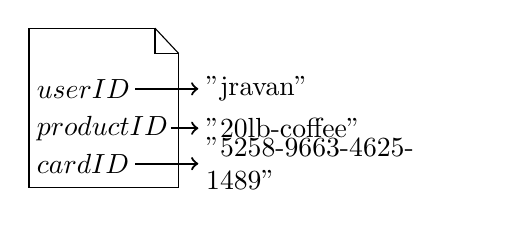
\begin{tikzpicture}
  \draw (0,0) -- (0,2.02) -- (1.6,2.02) -- (1.6,1.7) -- (1.9,1.7) -- (1.9,0) -- cycle;
  \draw (1.6,2.02) -- (1.9,1.7);
  \node[text width=1.5cm] at (.85,1.25) {$userID$};
  \node[text width=1.5cm] at (.85,.75) {$productID$};
  \node[text width=1.5cm] at (.85,.3) {$cardID$};
  \draw[thick,->] (1.35,1.25) -- (2.15,1.25);
  \draw[thick,->] (1.8,.75) -- (2.15,.75);
  \draw[thick,->] (1.35,.3) -- (2.15,.3);
  \node[text width=3.5cm] at (4,1.25) {"jravan"};
  \node[text width=3.5cm] at (4,.75) {"20lb-coffee"};
  \node[text width=3.5cm] at (4,.3) {"5258-9663-4625-1489"};
\end{tikzpicture}

\caption{e-Commerce Web Site Ticket Example} % title of the Figure
\label{fig:e_com_ticket} %% label to refer figure in text

\end{figure}

\begin{figure}[h]
\captionsetup{justification=centering}
\centering % used for centering Figure

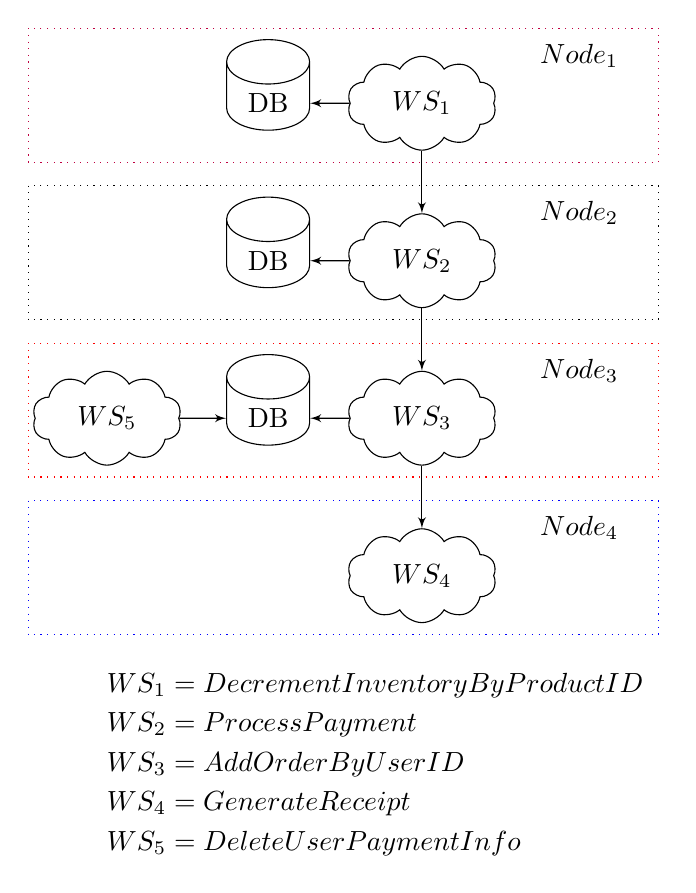
\begin{tikzpicture}
    \node [webservice, anchor=north] (ws4) {$WS_{4}$};
    \node [webservice, above=2cm of ws4.north, anchor=north] (ws3) {$WS_{3}$};
    \node [webservice, above=2cm of ws3.north, anchor=north] (ws2) {$WS_{2}$};
    \node [webservice, above=2cm of ws2.north, anchor=north] (ws1) {$WS_{1}$};
    \node [draw, cylinder, shape border rotate=90, aspect=0.75, %
      minimum height=30, minimum width=30, anchor=north, left=.5cm of ws3] (data3) {DB};
    \node [draw, cylinder, shape border rotate=90, aspect=0.75, %
      minimum height=30, minimum width=30, above=2cm of data3.north, anchor=north] (data2) {DB};
    \node [draw, cylinder, shape border rotate=90, aspect=0.75, %
      minimum height=30, minimum width=30, above=2cm of data2.north, anchor=north] (data1) {DB};
    \node [webservice, left=4cm of ws3.north, anchor=north] (ws5) {$WS_{5}$};
    \path [line] (ws1) -- (data1);
    \path [line] (ws2) -- (data2);
    \path [line] (ws3) -- (data3);
    \path [line] (ws1) -- (ws2);
    \path [line] (ws2) -- (ws3);
    \path [line] (ws3) -- (ws4);
    \path [line] (ws5) -- (data3);
    \draw[dotted,blue] (-5,.35) rectangle (3,-1.35);
    \draw[dotted,red] (-5,2.35) rectangle (3,.65);
    \draw[dotted,black] (-5,4.35) rectangle (3,2.65);
    \draw[dotted,purple] (-5,6.35) rectangle (3,4.65);
    \node[text width=1cm] at (2,6) {$Node_{1}$};
    \node[text width=1cm] at (2,4) {$Node_{2}$};
    \node[text width=1cm] at (2,2) {$Node_{3}$};
    \node[text width=1cm] at (2,0) {$Node_{4}$};
    \node[text width=7cm] at (-.5,-2) {$WS_{1} = Decrement Inventory By Product ID$};
    \node[text width=7cm] at (-.5,-2.5) {$WS_{2} = Process Payment$};
    \node[text width=7cm] at (-.5,-3) {$WS_{3} = Add Order By User ID$};
    \node[text width=7cm] at (-.5,-3.5) {$WS_{4} = Generate Receipt$};
    \node[text width=7cm] at (-.5,-4) {$WS_{5} = Delete User Payment Info$};
\end{tikzpicture}

\caption{Business Process for e-Commerce Web Site} % title of the Figure
\label{fig:bp_env} % label to refer figure in text

\end{figure}

Each dotted rectangle within Figure \ref{fig:bp_env} represents a distributed node containing a public web service executing transactions on an underlying database. In order for a successful purchase to take place within the e-commerce environment, the business process containing the web service sequence $WS_{1}, WS_{2}, WS_{3},$ and $WS_{4}$ must execute successfully. $WS_{1}$ ($DecrementInventoryByProductID$) uses the $productID$ provided from the current ticket in order to query the database regarding the requested product. This web service is responsible for searching the product and decrementing the number of items available for purchase. Once this task has been completed the ticket is passed off to $WS_{2}$. $WS_{2}$ ($ProcessPayment$) uses the payment information provided in the ticket to charge the user. If the payment is processed successfully, the ticket is forwarded to $WS_{3}$. $WS_{3}$ ($AddOrderByUserID$) is a service that takes the given $userID$, $product ID$, and creates a record of purchase history for the user. This allows the user to log in to their account at any time and see a record of their purchases. Once this has been processed successfully, it is handed off to $WS_{4}$ which is the final step in this purchase business process. $WS_{4}$ ($GenerateReceipt$) simply generates a receipt from the ticket information and is returned to the user's interface. A generated email with the attached receipt is also sent to the user for their own records. This web service does not require a database for its processing needs. Once $WS_{4}$ has completed processing, and only when it is finished, a purchase is considered successful.

The issue that arises in this situation is that web services can be executed by multiple hosts where the hosts are unaware of each others presence. This can cause issues for a node such as $Node_{3}$ where there are two different web services executing transactions on a single database instance. $WS_{3}$ and $WS_{5}$ provide two completely different services to requesting hosts, however the changes are reflected within the same database. $WS_{3}$ is a crucial part of the purchase business process in the provided use case but that does not mean that $WS_{3}$ can only be used in that process. In the event that both $WS_{3}$ and $WS_{5}$ are executed simultaneously, some type of concurrency control will need to be applied to retain consistency within the shared database. The next section will discuss the details of the two transactions that could potentially cause an inconsistent state along with cascading rollbacks throughout $Node_{1}$ and $Node_{2}$.

\subsection{Use Case Transactions for $Node_{3}$}

In Figure \ref{fig:webform} we see the contents of the two transactions executing on $Node_{3}$. $T_{DeleteUserPaymentInfo}$ is a transaction generated by $W_{5}$. The responsibility of this web service is to determine if the user exists and if they do exist, then to delete the user's payment information from the database by the provided \textit{userID}. $T_{AddOrderByUserID}$ is a transaction generated by $WS_{3}$ (mentioned above from Figure \ref{fig:bp_env}) that is responsible for adding an order record to a user account. $T_{AddOrderByUserID}$ executes under the pretext that the \textit{userID} given exists in the database or the web service would not have been able to be executed. If the \textit{userID}, does not exist then a new blank record will be created for the user and the order added to that record. If $T_{AddOrderByUserID}$ fails then an abort must be issued and all the previous operations committed from $WS_{1}$ and $WS_{2}$ must be rolled back. This includes operations that were executed from subsequent transactions that depended on the results of $WS_{1}$ and $WS_{2}$.

The two transactions executed from $WS_{3}$ and $WS_{5}$ consist of only two operations each. $T_{DeleteUserPaymentInfo}$ contains a single $R_{1}(b)$ and $W_{1}(b)$ where $b$ represents the user account associated with the given \textit{userID}. The transaction will first READ from the database to ensure the user exists and then WRITE out the user record if the user does exist\footnote{In this instance the WRITE operation executed would write a $NULL$ or empty record to the database in order to "delete" the record.}. The other transaction, $T_{AddOrderByUserID}$, also contains a single $R_{2}(b)$ and a single $W_{2}(b)$ where $b$ represents the order record to be persisted to the user's order history. The READ operation also ensures that the user exists first before the WRITE operation is executed. Each transaction contains a $C_{i}$ operation that represents the COMMIT operation that the database executes after all operations have completed. Figure \ref{fig:webform} shows the two transactions along with the operations contained within.

\begin{figure}[h]
\captionsetup{justification=centering}
\centering % used for centering Figure

\begin{picture}(50,40)
    \put(-70.5,25){$T_{AddOrderByUserID}$ = $R_{1}(b)W_{1}(b)C_{1}$}
    \put(-87,10){$T_{DeleteUserPaymentInfo}$ = $R_{2}(b)W_{2}(b)C_{2}$}
\end{picture}

\caption{e-Commerce Web Service Transaction Sequences} % title of the Figure
\label{fig:webform} % label to refer figure in text

\end{figure}

\subsection{Use Case Transaction Metrics}

For the transactions listed above, we know certain attributes regarding their executions including commit rate, number of transactions executed, and the execution time in regards to all transactions executing within the system. Commit rate is the percentage of successful commits over the total amount of attempted executions of that particular transaction. Number of transactions simply represents the total number of executions attempted (commits and aborts combined) for that particular transaction. Efficiency rate represents the average efficiency of the particular transaction to reach a completion state; whether it is a failure or success. A transaction with a very long execution time will have an efficiency rate that is much lower than a transaction that executes and completes very quickly. The attribute data listed above is consolidated into Table \ref{tbl:trans_metrics} below. 
\\
\begin{table}[h]
\captionsetup{justification=centering}
\centering
\begin{tabular}{|c|c|c|c|c|}
\hline
\multicolumn{4}{|c|}{\cellcolor[HTML]{EFEFEF}\textbf{Transaction Metrics}}                                                   \\ \hline
\textbf{Transactions} & \textbf{Commit Rate} & \textbf{\# of Transactions} & {\color[HTML]{000000} \textbf{Efficiency Rate}} \\ \hline
$T_{DeleteUserPaymentInfo}$         & 98\%                  & 200                         & 98\%                                          \\ \hline
$T_{AddOrderByUserID}$          & 97\%                     & 520                           & 99\%                                              \\ \hline
\end{tabular}

\caption{Transaction Metrics} % title of the Figure
\label{tbl:trans_metrics} % label to refer figure in text

\end{table}

In the scenario when the two transactions above are executed simultaneously, some form of concurrency control must be used to ensure that the database is left in a consistent state. In a web service context the isolation property will be relaxed and a serializable execution will be created. This serializable execution will be based on the conflicting operations of the two transactions. Figure \ref{fig:combined_history} displays an example of a generated serializable execution from $T_{AddOrderByUserID}$ and $T_{DeleteUserPaymentInfo}$.

\begin{figure}[h]
\captionsetup{justification=centering}
\centering % used for centering Figure

\begin{picture}(50,25)
    \put(-65,5){$T_{Serialized}$ = $R_{1}(b)W_{1}(b)R_{2}(b)W_{2}(b)C_{2}C_{1}$}
\end{picture}

\caption{Generated Serializable Execution} % title of the Figure
\label{fig:combined_history} % label to refer figure in text

\end{figure}

$T_{Serialized}$ is a well-formed serializable execution that does not violate any rules regarding conflicting operations. However, if $W_{2}(b)$ fails, a cascading rollback will be issued causing the operations of $T_{AddOrderByUserID}$ to be rolled back regardless of their successful execution. The operations of $T_{AddOrderByUserID}$ must be rolled back since they are a part of $T_{Serialized}$ and a COMMIT operation has not been executed yet. If $T_{AddOrderByUserID}$ was executed as a part of the business process outlined in the use case then the operations of the previous web services ($WS_{1}$ and $WS_{2}$) must be rolled back also.

Conversely, if the data in Table \ref{tbl:trans_metrics} were taken into consideration before generating the serializable execution, $T_{AddOrderByUserID}$ could be given a more restrictive concurrency control mechanism, such as traditional locking. Table \ref{tbl:trans_metrics} contains data that proves instances of $T_{AddOrderByUserID}$ have a high rate of commit with high percentage of efficiency throughout the system. Transactions with these properties could use traditional locking, execute in a serial manner, release locks in a short amount of time, and ensure the consistency of the database without causing other concurrent transactions from waiting. Table \ref{tbl:trans_metrics} also displays that instances of $T_{DeleteUserPaymentInfo}$ could use traditional locking techniques due to its history. Therefore $T_{AddOrderByUserID}$ and $T_{DeleteUserPaymentInfo}$ could execute serially using traditional locking techniques, commit changes quickly and successfully, and prevent a cascading rollback from reverting the effects of $WS_{1}$ and $WS_{2}$ just by using the reputation provided by the separate transactions. The next section will discuss the existing research that has taken place to remediate this problem without the current knowledge of transaction metrics.

\section{Existing Research}
Ensuring successful concurrency control in web service transactions has been studied in depth for some time(e.g., \cite{Fekete_Promises}, \cite{Fekete_IsolationSupport}, and \cite{Alrifai_Distributed_Managment}). The Promises model presented by Alan Fekete et al (e.g., \cite{Fekete_Promises} and \cite{Fekete_IsolationSupport}) is an elegant solution that "promises" a particular transaction that the requested resource will be available while allowing concurrent transactions to still execute on that resource. The Promises solution is robust in that it allows the "strengthening" or "weakening" of promises after they have already been made. This allows existing promises on resources to be modified without breaking the existing promise entirely. However, the solution introduces backwards compatibility issues along with a potential bottleneck at the occurrence of registering a promise for a particular transaction.

Alomari et all present a solution involving an External Lock Manager (ELM) that resides outside of the DBMS \cite{Fekete_SnapshotIso}. This allows a layer of separation between the application and the DBMS in order to schedule transactions using special business logic according to the environment. This is very similar to the approach taken with the Transaction Metrics logical unit within the solution presented in this paper; however, this solution lacks the prediction logic used to improve the consistency normally found in web service environments while also improving the performance lacking in traditional locking environments.

In the solution presented by Alrifai et al \cite{Alrifai_Distributed_Managment} an edge chasing solution using dependency graphs are incorporated in order to detect dependencies between globally scheduled transactions. The solution was tested parallel to the well known 2-Phase Locking Protocol (2PL) and provided promising results regarding efficiency. However, the Alrifai et al solution becomes less efficient when the number of dependency cycles are detected therefore rendering the solution's scalability mute and only useful in small environments. 

The model of the different lock types comes from Christian Jacobi et al with their research in concurrent locking with parallel database systems \cite{Jacobi_Locking}. The researchers extended the use of the native lock types in the existing database structure in order to speed up thread processing on multi-processor machines. This extension of the locking mechanisms is the basis of our new approach to increasing concurrent transactions while keeping the database in a consistent state. 

Prediction-based concurrency control has been proposed by Eunhee Lee et al with the entity-radius solution \cite{Eunhee_PredictionBasedCC}. This solution uses the concept of multiple entity radii that attempts to predict the next user based on their location. The prediction is generated from the location within a radius of the replicated site and their navigation speed. The solution provided is elegant with excellent experimental results but no formal proof or analysis of the algorithm is provided. The solution is also based solely on virtual game environments rather than BPEL business processes. 

Other solutions to prevent business process cancellation or rollback when participants of the process do not behave correctly involve global views of the process \cite{Riegen_RuleBased}, \cite{Fekete_RAMP}. Support for these types of solutions are based on the well-known Oasis specifications of WS-Coordination, WS-AtomicTransaction, and WS-BusinessActivity \cite{WSCO}, \cite{WSAT}, \cite{WSBA}. These solutions are well-designed however they require the presence of a global coordinator throughout the entire process of a business process. A local solution that is independent of coordination is much more extensible and flexible for an continuously growing web service environment. The next section will discuss the system model generated from the current available work with the prediction-based solution.


\section{System Model}
This section outlines the system model on which the solution is built. Definitions for existing and new concepts are introduced first considering they will be used to describe the different components that consist of the system model. Later subsections explain in detail the different components and processes required for the prediction-based solution.

\subsection{Definitions}
\label{definitions}

\begin{definition}
\label{cmt_rate}
 (Commit Rate) - commit rate is calculated by the given formula:
 
 \[\textrm{$c$} = \textrm{\# of executions ending with a COMMIT result}\]
 \[\textrm{$a$} = \textrm{\# of executions ending with a ABORT result}\]
 \[\textrm{\textit{Commit Rate}} =\frac{\abs{c}}{\abs{c + a}}\]
 
 Once this ratio is calculated it is compared to the overall ratio of commit to abort executions for all transactions.
 
\end{definition}

\begin{definition}
\label{eff_rate}
 (Efficiency Rate) - efficiency rate is based on how its execution time compares to all transactions executed within the execution environment. The efficiency rate is calculated based on the given formula:
 
\[\textrm{\textit{Efficiency Rate}} =\frac{\textrm{$AVG(AVG(T_{1}),...,AVG(T_{n}))$}}{\textrm{$AVG(T_{i})$}}\]
 
\end{definition}

\begin{definition}
\label{cat_bounds}
 (Categorization Bounds) - categorization bounds are upper and lower limits of both commit rate and efficiency rate that are used when categorizing transactions. These are put in place to prevent any particular transaction category from potentially covering the entire categorization graph. The categorization bounds are static values that do not change throughout the system execution. Both the efficiency rate and the commit rate bounds are currently at 50\% creating full coverage of all transactions.
\end{definition}

% \begin{definition}
% \label{cat_threshold}
%  (Categorization Thresholds) - categorization thresholds are calculated within the categorization bounds (see Definition \ref{cat_bounds}) by using the Transaction Concentration Ratio (see Section \ref{sec:TCR}). The threshold values are dynamic and change depending on the execution environment but will not exceed the categorization bounds placed on that particular category. Categorization thresholds enforce the most accurate thresholds for the execution environment while allowing flexibility.
% \end{definition}

\begin{definition}
\label{min_commit}
(HCHE) - HCHE, acronym for High Commit High Efficiency, is a transaction categorization with categorization bounds (see Definition \ref{cat_bounds}) that involve a commit rate of 50\% and higher and a efficiency rate in the upper 50\% and higher as well (see Definitions \ref{cmt_rate} and \ref{eff_rate}). Table \ref{tbl:default_tmetrics} outlines all transaction categories.
\end{definition}

\begin{definition}
\label{min_abrt}
(LCHE) - LCHE, acronym for Low Commit High Efficiency, is a transaction categorization with categorization bounds (see Definition \ref{cat_bounds}) that involve a commit rate of 50\% and lower and a efficiency rate in the upper 50\% and higher (see Definitions \ref{cmt_rate} and \ref{eff_rate}). Table \ref{tbl:default_tmetrics} outlines all transaction categories.
\end{definition}

\begin{definition}
\label{ext_commit}
(HCLE) - HCLE, acronym for High Commit Low Efficiency, is a transaction categorization with categorization bounds (see Definition \ref{cat_bounds}) that involve a commit rate of 50\% and higher and a efficiency rate in the bottom 50\% and lower (see Definitions \ref{cmt_rate} and \ref{eff_rate}). Table \ref{tbl:default_tmetrics} outlines all transaction categories.
\end{definition}

\begin{definition}
\label{ext_abrt}
(LCLE) - LCLE, acronym for Low Commit Low Efficiency, is a transaction categorization with categorization bounds (see Definition \ref{cat_bounds}) that involve a commit rate of 50\% and lower and a efficiency rate in the bottom 50\% and lower as well (see Definitions \ref{cmt_rate} and \ref{eff_rate}). Table \ref{tbl:default_tmetrics} outlines all transaction categories.
\end{definition}

%\begin{definition}
%\label{no_trend}
%(NO\_TREND) - NO\_TREND is a transaction categorization with categorization bounds (see Definition \ref{cat_bounds}) that include all %the outlining space that the previous four categories do not include. If the efficiency rate is less than or equal to 25\% then the %commit rate must be between 25\% and 75\% (see Definitions \ref{cmt_rate} and \ref{eff_rate}). If the efficiency rate is between 25\% %and 75\% then the commit rate includes all values ranging from 0\% to 100\%. Finally, if the efficiency rate is greater than or equal %to 75\% then the commit rate must be between 25\% and 75\%. Table \ref{tbl:default_tmetrics} outlines all transaction categories.
%\end{definition}

\begin{table}[h]
\captionsetup{justification=centering}
\centering
\begin{tabular}{l|c|c|}
\cline{2-3}
                                          & \multicolumn{1}{l|}{\textbf{Efficiency Rate ($E_{r}$)}} & \multicolumn{1}{l|}{\textbf{Commit Rate ($C_{r}$)}} \\ \hline
\multicolumn{1}{|l|}{\textbf{HCLE}}  & $\le$ 50\%                       & $\ge$ 50\%                               \\ \hline
\multicolumn{1}{|l|}{\textbf{LCLE}} & $\le$ 50\%                       & $\le$ 50\%                                 \\ \hline
\multicolumn{1}{|l|}{\textbf{HCHE}}  & $\ge$ 50\%                          & $\ge$ 50\%                                \\ \hline
\multicolumn{1}{|l|}{\textbf{LCHE}} & $\ge$ 50\%                          & $\le$ 50\%                                  \\ \hline
%\multicolumn{1}{|l|}{\textbf{No Trnd.}} &    \multicolumn{2}{c|}{See equation below}                                    \\ \hline
\end{tabular}
\caption{Transaction Categorization Bounds} % title of the Figure
\label{tbl:default_tmetrics} % label to refer figure in text
\end{table}

%\[
%\left \{
%  \begin{tabular}{ll}
%  
%  $E_{r}\le25\%$, & $25\%<C_{r}<75\%$ \\
%  $25\%<E_{r}<75\%$, & $0\%\le C_{r}\le100\%$ \\
%  $E_{r}\ge75\%$, & $25\%<C_{r}<75\%$
%  
%  \end{tabular}
%\right \}
%\]

\begin{definition}
\label{conflict_ops}
 (Conflicting Operations) - two operations are considered conflicting if they contain all of the following attributes:

 \begin{enumerate}
   \item both are contained within different transactions
   \item both operations are operating on the same data item
   \item and at least one of the operations is a WRITE
 \end{enumerate}

 \begin{example}
 \label{ex_conflict_ops}
  $o_{1}$ is a READ operation on resource $R_{User ID}$ in $T_{1}$ and $o_{2}$ is a WRITE operation on $R_{User ID}$ in    $T_{2}$. These two operations are considered conflicting.
 \end{example}
\end{definition}

\begin{definition}
\label{conflict_trans}
 (Conflicting Transactions) - two transactions are considered conflicting if they contain all of the following attributes:
 
 \begin{enumerate}
 \item both transactions contain conflicting operations (see Definition \ref{conflict_ops})
 \item both transactions are contained within the same serializable schedule
 \item and at least one of the transactions is categorized to abort
 \end{enumerate}
 
 \begin{example}
 \label{ex_conflict_trans}
  Using the transactions mentioned in Example \ref{ex_conflict_ops} let's say the serializable schedule $S_{1}$ contains   an interleaved execution of $T_{1}$ and $T_{2}$. These transactions are now considered conflicting.
 \end{example}
\end{definition}

\begin{definition}
\label{conflict_cat}
  (Conflicting Categories) - conflicting categories are very much related to conflicting transactions (see Definition \ref{conflict_trans}) however this definition is concerned with the categories the transactions have been placed in rather than the transactions themselves. Two categories are said to be conflicting if they contain all of the following attributes:
  
  \begin{enumerate}
  \item both are contained within the same serializable schedule
  \item and at least one of the categories is predicted to abort
  \end{enumerate}
  
Transactions of conflicting categories are not allowed within the same schedule within this solution.  
  
  \begin{example}
  For example, let's say we have transaction $T_{1}$ that has been placed in the category HCHE and transaction $T_{2}$ that has been placed in the category LCLE. These two categories are considered conflicting even if $T_{1}$ and $T_{2}$ are not considered to be conflicting transactions themselves.
  \end{example}
  
\end{definition}

\begin{definition}
\label{serial_sched}
 (Serializable Schedule) - a serializable schedule is a non-serial schedule that can be converted to a serial schedule by interchanging non-conflicting operations (see Definition \ref{conflict_ops})

\end{definition}

\begin{definition}
\label{casc_rollback}
 (Cascading Rollback) - a cascading rollback occurs when two conflicting transactions (see Definition                     \ref{conflict_trans}) are interleaved within the same serializable schedule. The abort is cascading in the sense that an  abort must be issued for each transaction within the schedule that was dependant upon the transaction that issued the abort. This is needed to ensure a consistent state within the database.
 
 \begin{example}
 \label{ex_casc_rollback}
  Using the serializable schedule generated in Example \ref{ex_conflict_trans}, if transaction $T_{2}$ issues an abort then  transaction $T_{1}$ must also be aborted since $T_{1}$ is dependant upon $T_{2}$.
 \end{example}
 
\end{definition}

\begin{definition}
\label{grant_action}
 (Grant Action) - the grant action is one of the three possible actions that can take place within the two lock compatibility matrices (Table \ref{tbl:read_lock_compatibility} \& Table \ref{tbl:write_lock_compatibility}). This action is represented by the plus sign (+) which signifies that there is not a conflict between the granted and requesting transactions and the lock can be granted to the transaction that is requesting access to the resource.
 
 \begin{example}
 \label{ex_grant_action}
  A read-lock for a resource $R$ has been granted to transaction $T_{1}$ within the $HCHE$ transactional category. Transaction $T_{2}$ within the $HCLE$ is also requesting a read-lock to resource $R$. This does not cause a conflict and therefore the grant action will be taken and the requested lock will be issued to $T_{2}$.
 \end{example}
 
\end{definition}

\begin{definition}
\label{decline_action}
 (Decline Action) - the decline action is one of the three possible actions that can take place within the two lock compatibility matrices (Table \ref{tbl:read_lock_compatibility} \& Table \ref{tbl:write_lock_compatibility}). This action is represented by the minus sign (-) which signifies that there is a conflict between the granted and requesting transactions and the lock can not be granted to the transaction that is requesting access to the resource.
 
 \begin{example}
 \label{ex_decline_action}
  A write-lock for a resource $R$ has been granted to transaction $T_{1}$ within the $HCHE$ transactional category. Transaction $T_{2}$ within the $HCLE$ is requesting a write-lock to resource $R$. This causes a conflict and therefore the decline action will be taken and the requested lock will not be issued to $T_{2}$.
 \end{example}
 
\end{definition}

\begin{definition}
\label{elevate_action}
 (Elevate Action) - the elevate action is one of the three possible actions that can take place within the two lock compatibility matrices (Table \ref{tbl:read_lock_compatibility} \& Table \ref{tbl:write_lock_compatibility}). This action is represented by the delta symbol ($\delta$) which signifies that the transaction requesting access to the resource is in a category that contains a higher prioritization (see Table \ref{tbl:priority}) than the transaction that currently holds the lock to the resource.
 
 \begin{example}
 \label{ex_elevate_action}
  A read-lock for a resource $R$ has been granted to transaction $T_{1}$ within the $LCLE$ transactional category. Transaction $T_{2}$ within the $HCHE$ is requesting a write-lock to resource $R$. This causes a conflict however since $T_{2}$ contains a higher priority than $T_{1}$ the elevate action will be taken and the requested lock will be issued to $T_{2}$.
 \end{example}
 
\end{definition}

\subsection{Environment}
In a web services environment multiple web services can submit transactions to a database to be executed. As mentioned before, if only one transaction can be executed at any given time then other concurrent transactions from other web services must wait. This causes a huge performance degradation, therefore concurrent transactions from multiple web services must be handled. This is where the Database Management System's (DBMS) scheduler plays an important role in ensuring concurrent transactions preserve consistency within the database. The scheduler receives transactions that are submitted from web services and generates a serializable schedule based on the conflicting operations contained within the transactions. 

After receiving the concurrent transactions (e.g., $T_{1}$, $T_{2}$, ... , $T_{N}$) the scheduler is responsible for analyzing the conflicting operations within the transactions and generating a serializable schedule that will then be executed on the database itself (e.g., $T_{Sched}$). This serializable execution is guaranteed to leave the database in a consistent state after a successful execution due to the analysis performed by the scheduler and the ordering of the operations within the transaction. Figure \ref{fig:Tsched} displays the generation of $T_{Sched}$ from multiple web service transactions. Figure \ref{fig:ws_env} displays a diagram of the database scheduler in a web service context.

\begin{figure}[h]
\captionsetup{justification=centering}
\centering % used for centering Figure

\begin{picture}(55,100)
    \put(-93,80){$T_{1}$ = \{ $W_{1}(r_{1})R_{1}(r_{1})W_{1}(r_{2})R_{1}(r_{2})$ ... $W_{1}(r_{n})R_{1}(r_{n})C_{1}$ \}}
    \put(-93,65){$T_{2}$ = \{ $W_{2}(r_{1})R_{2}(r_{1})W_{2}(r_{2})R_{2}(r_{2})$ ... $W_{2}(r_{n})R_{2}(r_{n})C_{2}$ \}}
    \put(-58,50){.}
    \put(-58,45){.}
    \put(-58,40){.}
    \put(-100,23){$T_{N}$ = \{ $W_{n}(r_{1})R_{n}(r_{1})W_{n}(r_{2})R_{n}(r_{2})$ ... $W_{n}(r_{n})R_{n}(r_{n})C_{N}$ \}}
    \put(-100,18){\makebox[\linewidth]{\rule{8.5cm}{0.4pt}}}
    \put(-90,5){$T_{Sched}$ = \{ $T_{1}T_{2}$ ... $T_{N}$ \}}
\end{picture}

\caption{Generation of $T_{Sched}$ from Concurrent Web Service Transactions} % title of the Figure
\label{fig:Tsched} % label to refer figure in text

\end{figure}

\begin{figure}[h]
\captionsetup{justification=centering}
\centering % used for centering Figure

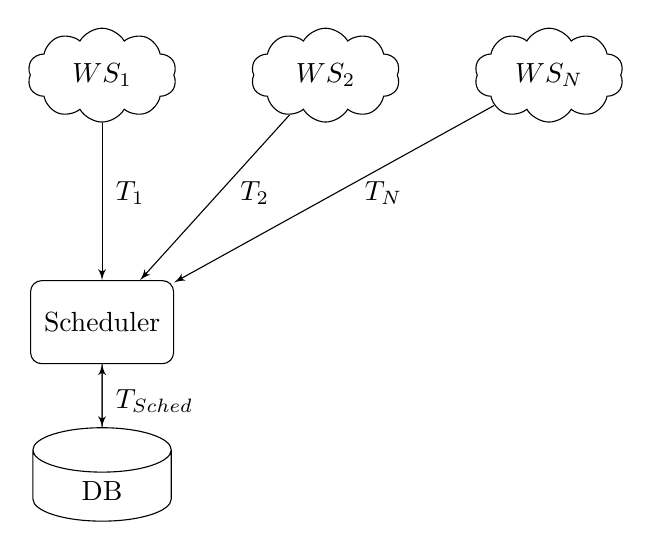
\begin{tikzpicture}
    \node [draw, cylinder, shape border rotate=90, aspect=0.75, %
      minimum height=30, minimum width=50] (data) {DB};
    \node [block, above=2cm of data.south,anchor=south] (sched) {Scheduler};
    \node [webservice, above=2cm of sched] (ws1) {$WS_{1}$};
    \node [webservice, right=of ws1] (ws2) {$WS_{2}$};
    \node [webservice, right=of ws2] (wsN) {$WS_{N}$};
    \path [line] (sched) -- (data);
    \path [line] (data) -- (sched);
    \path [line] (ws1) -- (sched);
    \path [line] (ws2) -- (sched);
    \path [line] (wsN) -- (sched);
    \put(5,105){$T_{1}$}
    \put(50,105){$T_{2}$}
    \put(95,105){$T_{N}$}
    \put(5,30){$T_{Sched}$}
\end{tikzpicture}

\caption{Web Service Environment with Scheduler} % title of the Figure
\label{fig:ws_env} % label to refer figure in text

\end{figure}

The architecture shown in Figure \ref{fig:ws_env} is a typical web service environment that exists currently. The existing web service environment treats all transactions equally. Every transaction submitted to the DBMS scheduler is compiled into a serializable execution and submitted to the database. The drawback of this type of architecture is the case of a cascading rollback. In the event of a cascading rollback, operations that have successfully completed must be reverted due to the failure of a dependant operation in a separate transaction. The prediction-based architecture used in this solution adds a new logical component (Transaction Metrics). This component is added at the scheduling level to analyze certain metadata about transactions submitted to the scheduler. Table \ref{tbl:trans_metrics} displays the type of data that will be calculated in order to make an accurate prediction on the likelihood that a transaction will either commit or abort. Once implemented, transactions will build a history, or a reputation, based on commit rate and efficiency rate. The Transaction Metrics logical unit will store this data within the database instance itself. Transactions executing from this component ($T_{Metrics}$) can use traditional locking techniques since it is known that no other web service transactions will be conflicting with these transactions. The relation used to store this metric data will be known only to the internal components of this database instance; not outside web services. Figure \ref{fig:ws_env_with_metrics} displays the addition to the existing architecture in the prediction-based solution.

\subsection{Transaction Categorization}

In order to ensure that correct lock techniques are selected, transactions cannot be simply characterized as good or bad based on their metrics. For example, a transaction $T_{1}$ may have a 100\% commit rate but it has a long execution time. A transaction with these characteristics should not be penalized when in fact it is a well behaving transaction. On the other hand, a transaction $T_{2}$ that has a 100\% commit rate and has an extremely short execution time should not be treated with the same priority as $T_{1}$. This is where certain of levels must be established to ensure the most appropriate selection is made.

In order to establish levels, there were different categorizations where the transactions were placed in. The first categorization is based solely on the efficiency of the transaction. In this categorization, there are two attributes: \textit{high efficiency (HE)} and \textit{low efficiency (LE)}. A transaction that has been labeled as \textit{HE} is considered to execute with an efficiency in the upper 50\% of all transactions executed within the system\footnote{See Section \ref{section_cat_graph} and Section \ref{definitions} for more clarification}. The second attribute, \textit{LE}, is any transaction where its efficiency rate is in the lower 50\% of all transactions executed. These transactions will consist of the majority of transactions that are going to execute on the database. Transactions of this nature could potentially execute on the system for days or could be a long running BPEL transaction \cite{BPEL}.

The second categorization that the levels are built on is based solely on the outcome of the transaction. These attributes are \textit{high commit (HC)} and \textit{low commit (LC)} which are much more simple to define. A transaction with a \textit{HC} attribute has committed successfully over 50\% of executions and persisted to disk (upper 50\% of all transactions). A transaction with an \textit{LC} attribute has failed over 50\% of its executions and has not persisted to disk (lower 50\% of all transactions). This categorization correlates directly with the commit rate defined (see Definition \ref{cmt_rate}).

With these two categorizations and two attributes a four-level system was devised in order to select appropriate lock types. The four categories devised are \textit{high commit-high efficiency (HCHE)}, \textit{high commit-low efficiency (HCLE)}, \textit{low commit-high efficiency (LCHE)}, and \textit{low commit-low efficiency (LCLE)}. Depending on the level in which the transaction has been placed, different lock types will be granted in order to perform concurrency control. The next section will discuss the compatibility of the lock types among transactional categories.

\subsection{Lock Compatibility Among Transaction Categories}

There are two main lock types when it comes to lock types in a DBMS: shared read-locks and exclusive write-locks. Shared read-locks allow read access to resource, \textit{R}, to be accessed by multiple parties. \textit{R} can be a relation, tuple, or even an individual cell in a database, depending on the lock granularity set by the system. Exclusive write-locks only allow write access to the particular resource for the transaction that holds the lock. This is considered a binary lock. At any point in time in the execution of multiple concurrent transactions, there is only one exclusive write-lock per resource and only the lock holder can manipulate the data.

%Based on Fekete's pre-emptive priority scheduling
To improve the performance of the system during the execution of concurrent transactions, we force lower priority transactional categories to release locks to higher priority categories. This allows transactions with a better reputation to execute more quickly while transactions with a poor reputation do not create a bottleneck for later transactions. This process increases throughput for transactional execution while preserving the consistency of the database through traditional locking. In order to successfully prioritize transactions, an objective priority was placed on each of the four transactional categories mentioned above. Table \ref{tbl:priority} displays the priorities that are used to make these decisions.

\begin{table}[h]
\captionsetup{justification=centering}
\centering
\begin{tabular}{l|c|}
\cline{2-2}
                                          & \multicolumn{1}{l|}{\textbf{Priority}} \\ \hline
\multicolumn{1}{|l|}{\textbf{HCHE}}  & I                                      \\ \hline
\multicolumn{1}{|l|}{\textbf{HCLE}}  & II                                     \\ \hline
\multicolumn{1}{|l|}{\textbf{LCHE}} & III                                     \\ \hline
\multicolumn{1}{|l|}{\textbf{LCLE}} & IV                                      \\ \hline
\end{tabular}

\caption{Category Priorities} % title of the Figure
\label{tbl:priority} % label to refer figure in text

\end{table}

There are two compatibility matrices that were created as a result of the four transactional categories and two lock types. These matrices explicitly define the actions that should be taken when transactional categories request locks to the resources that have already granted locks.\footnote{In the event that a lock is requested of a resource that has not issued any locks, then the lock will be automatically granted. There is no conflict and therefore the compatibility matrices do not apply.} The actions defined within the matrices are derived based on the category prioritization made in Table \ref{tbl:priority}. Table \ref{tbl:read_lock_compatibility} displays the lock compatibility for all transactional categories where a read-lock has already been granted. Table \ref{tbl:write_lock_compatibility} displays the lock compatibility for all transactional categories where a write-lock has already been granted. There are three actions that can be taken in regards to the lock compatibility matrix: \textit{grant action} (see Definition \ref{grant_action}), \textit{decline action} (see Definition \ref{decline_action}), and \textit{elevate action} (see Definition \ref{elevate_action}). The combination of these actions within the DBMS ensure consistency for transactions but they also prevent transactions with bad reputations from holding up transactions with good reputations.

By using the four levels defined above for determining the level in which a transaction is placed, we can more appropriately determine the concurrency control mechanism needed rather than using a "one size fits all" approach for all transactions entering the system. The next section will address the issue of multiple locks that are granted for a single resource.

\begin{table}[h]
\captionsetup{justification=centering}
\centering
\begin{tabular}{l|c|c|c|c|c|c|}

\cline{2-5} & 
\multicolumn{4}{c|}{\textbf{already granted lock}} \\

\cline{2-5} \hline

\multicolumn{1}{|l|}{\begin{tabular}[c]{@{}c@{}}\textbf{requested}\\\textbf{lock}\end{tabular}} &\textbf{$HCHE_{r}$}    & \textbf{$HCLE_{r}$}    & \textbf{$LCHE_{r}$}     & \textbf{$LCLE_{r}$}    \\ \hhline{=#====}
\multicolumn{1}{|l||}{\textbf{$HCHE_{r}$}} &\textbf{+}    & \textbf{+}    & \textbf{+}     & \textbf{+}    \\ \hline
\multicolumn{1}{|l||}{\textbf{$HCLE_{r}$}} &\textbf{+}    & \textbf{+}    & \textbf{+}     & \textbf{+}    \\ \hline
\multicolumn{1}{|l||}{\textbf{$LCHE_{r}$}} &\textbf{+}    & \textbf{+}    & \textbf{+}     & \textbf{+}    \\ \hline
\multicolumn{1}{|l||}{\textbf{$LCLE_{r}$}} &\textbf{+}    & \textbf{+}    & \textbf{+}     & \textbf{+}    \\ \hline
\multicolumn{1}{|l||}{\textbf{$HCHE_{w}$}} &\textbf{-}    & $\delta$      & $\delta$       & $\delta$        \\ \hline
\multicolumn{1}{|l||}{\textbf{$HCLE_{w}$}} &\textbf{-}    & \textbf{-}    & $\delta$       & $\delta$        \\ \hline
\multicolumn{1}{|l||}{\textbf{$LCHE_{w}$}} &\textbf{-}    & \textbf{-}    & \textbf{-}     & $\delta$        \\ \hline
\multicolumn{1}{|l||}{\textbf{$LCLE_{w}$}} &\textbf{-}    & \textbf{-}    & \textbf{-}     & \textbf{-}    \\ \hline           
\end{tabular}

\caption{Read-Lock Compatibility} % title of the Figure
\label{tbl:read_lock_compatibility} % label to refer figure in text

\end{table}


\begin{table}[h]
\captionsetup{justification=centering}
\centering
\begin{tabular}{l|c|c|c|c|c|c|}

\cline{2-5} & 
\multicolumn{4}{c|}{\textbf{already granted lock}} \\

\cline{2-5} \hline

\multicolumn{1}{|l|}{\begin{tabular}[c]{@{}c@{}}\textbf{requested}\\\textbf{lock}\end{tabular}} &\textbf{$HCHE_{w}$}    & \textbf{$HCLE_{w}$}    & \textbf{$LCHE_{w}$}     & \textbf{$LCLE_{w}$}    \\ \hhline{=#====}
\multicolumn{1}{|l||}{\textbf{$HCHE_{r}$}} &\textbf{-}    & \textbf{-}    & \textbf{-}     & \textbf{-}    \\ \hline
\multicolumn{1}{|l||}{\textbf{$HCLE_{r}$}} &\textbf{-}    & \textbf{-}    & \textbf{-}     & \textbf{-}    \\ \hline
\multicolumn{1}{|l||}{\textbf{$LCHE_{r}$}} &\textbf{-}    & \textbf{-}    & \textbf{-}     & \textbf{-}    \\ \hline
\multicolumn{1}{|l||}{\textbf{$LCLE_{r}$}} &\textbf{-}    & \textbf{-}    & \textbf{-}     & \textbf{-}    \\ \hline
\multicolumn{1}{|l||}{\textbf{$HCHE_{w}$}} &\textbf{-}    & $\delta$      & $\delta$       & $\delta$        \\ \hline
\multicolumn{1}{|l||}{\textbf{$HCLE_{w}$}} &\textbf{-}    & \textbf{-}    & $\delta$       & $\delta$        \\ \hline
\multicolumn{1}{|l||}{\textbf{$LCHE_{w}$}} &\textbf{-}    & \textbf{-}    & \textbf{-}     & $\delta$        \\ \hline
\multicolumn{1}{|l||}{\textbf{$LCLE_{w}$}} &\textbf{-}    & \textbf{-}    & \textbf{-}     & \textbf{-}    \\ \hline           
\end{tabular}

\caption{Write-Lock Compatibility} % title of the Figure
\label{tbl:write_lock_compatibility} % label to refer figure in text

\end{table}

\subsection{Resource Category Data Structure}
\label{RCDS}

In Table \ref{tbl:read_lock_compatibility} there are multiple \textit{grant actions} (see Definition \ref{grant_action}) which could potentially cause multiple read-locks to be granted for a single resource. It is appropriate for a resource to grant multiple read-locks however in order to properly handle the \textit{elevate actions} the comparison must be made with the granted lock of the highest priority. For example, a resource $R_{a}$ has granted two read-locks to transactions $T_{1}$ and $T_{2}$ with categories $HCLE_{r}$ and $LCLE_{r}$. While these two locks are still granted a transaction $T_{3}$ categorized as $HCLE$ requests a write-lock $HCLE_{w}$ to $R_{a}$. If the evaluation based on Table \ref{tbl:read_lock_compatibility} is completed by using the read-lock granted to $T_{2}$ then an \textit{elevate action} would be issued since the requesting lock contains a higher priority than the granted lock. However, if the evaluation is completed by using the read-lock granted to $T_{1}$ then a \textit{decline action} would be issued since the requesting lock contains a priority of equal standing with the granted lock.

When situations such as this arise in the system, the evaluation completed  in the compatibility matrix should be completed against the granted lock with the highest priority. By evaluating against the granted lock whose transaction has been categorized with the highest priority, this prevents starvation of transactions with categorizations of lower priority. Using the example illustrated above, if the comparison was completed with transaction $T_{2}$ instead, then an \textit{elevate action} would be issued and transaction $T_{2}$ would be preemptively aborted and caused to compete for the lock again. If transactions are continually submitted to the system that are categorized with a higher priority than $T_{2}$ then $T_{2}$ will continually be aborted or overlooked and will never successfully complete.

In order to ensure that Table \ref{tbl:read_lock_compatibility} is used with the transaction categorized with the highest priority, a new data structure is introduced. This data structure is used in order to maintain knowledge of all granted locks for a particular resource. It also allows efficient access to the lock with the highest priority for comparisons. The data structure is a combination of two established data structures used throughout computer science: linked list and min-heap (min-priority queue). The first part of the data structure, the linked list, contains all resources in the system that have a read-lock granted\footnote{This data structure only applies to read-locks in Table \ref{tbl:read_lock_compatibility}. Table \ref{tbl:read_lock_compatibility} is the only compatibility matrix that contains \textit{grant actions} and therefore only read-locks can cause a lock comparison conflict within the matrix}. It is a linear singly-linked list to allow processing in one direction. Each node in the linked list has a single reference to the root node of a min-heap. The min-heap contains all granted locks for the resource that has a reference to the min-heap root node. The min-heap property is calculated by the category priority of the locks that are granted. Since the highest priority, as shown in Table \ref{tbl:priority}, is represented by the lowest integer value, then the lock with the highest priority will make its way to the root node of the min-heap by nature of min-heap properties \cite[p.162]{Cormen_Algorithms}. This accommodates efficient processing for accessing the highest priority of all locks granted to a particular resource. More details of how the Resource Category Data Structure is used are outlined in Section \ref{sec:algorithms}. Figure \ref{fig:resource_cat_structure} displays a graphical representation of the Resource Category Data Structure.

\begin{figure}[ht]  
\captionsetup{justification=centering}
\centering % used for centering Figure

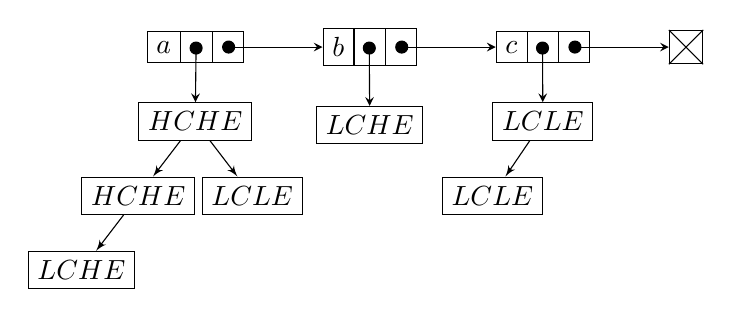
\begin{tikzpicture}
    [list/.style={rectangle split, rectangle split parts=3,
    draw, rectangle split horizontal}, >=stealth, start chain]

  \node[list,on chain] (A) {$a$};
  \node[list,on chain] (B) {$b$};
  \node[list,on chain] (C) {$c$};
  \node[rectangle, draw, below=.5cm of A] (HCHE1){$HCHE$};
  \node[rectangle, draw, below=.7cm of HCHE1.west] (HCHE2){$HCHE$};
  \node[rectangle, draw, below=.7cm of HCHE1.east] (LCLE1){$LCLE$};
  \node[rectangle, draw, below=.7cm of HCHE2.west] (LCHE1){$LCHE$};
  \node[rectangle, draw, below=.5cm of B] (LCHE2){$LCHE$};
  \node[rectangle, draw, below=.5cm of C] (LCLE2){$LCLE$};
  \node[rectangle, draw, below=.7cm of LCLE2.west] (LCLE3){$LCLE$};
  \node[on chain,draw,inner sep=6pt] (D) {};
  \draw (D.north east) -- (D.south west);
  \draw (D.north west) -- (D.south east);
  \draw[*->] let \p1 = (A.two), \p2 = (A.center) in (\x1 + 2,\y2 + 2) -- (HCHE1);
  \draw[*->] let \p1 = (B.two), \p2 = (B.center) in (\x1 + 2,\y2 + 2) -- (LCHE2);
  \draw[*->] let \p1 = (C.two), \p2 = (C.center) in (\x1 + 2,\y2 + 2) -- (LCLE2);
  \draw[*->] let \p1 = (A.three), \p2 = (A.center) in (\x1,\y2) -- (B);
  \draw[*->] let \p1 = (B.three), \p2 = (B.center) in (\x1,\y2) -- (C);
  \draw[*->] let \p1 = (C.three), \p2 = (C.center) in (\x1,\y2) -- (D);
  \path [line] (HCHE1) -- (HCHE2);
  \path [line] (HCHE1) -- (LCLE1);
  \path [line] (HCHE2) -- (LCHE1);
  \path [line] (LCLE2) -- (LCLE3);
  
\end{tikzpicture}

\caption{Resource Category Data Structure} % title of the Figure
\label{fig:resource_cat_structure} % label to refer figure in text

\end{figure}

\subsection{Transaction Conflict Resolution}

Although the transactions will receive a level of categorization when submitted to the scheduler there has to be some mechanism in place in order to handle the conflicting categorizations (see Section \ref{conflict_cat}).  When two transactions are submitted to execute concurrently with this property they must be executed serially rather than concurrently to  maintain the consistency of the database. If two conflicting transactions were executed concurrently then one aborted operation in either of the two transactions would cause an inconsistent state. A cascading rollback would have to occur in order to re-establish consistency within the database.

In order to choose which transaction is executed first in the serial execution of two conflicting categories, a priority system was needed. For this priority system, the categorization priorities outlined in Table \ref{tbl:priority} were used just as they were used in the lock compatibility matrices. For example, if two transactions are submitted to the scheduler to execute concurrently but neither are predicted to abort then no conflict is detected. The two transactions will execute concurrently, commit successfully, and consistency is preserved in the database. However, if one of the transactions is predicted to abort, then this transaction could potentially affect the outcome of the successful transaction. In this situation we want to preserve consistency and therefore the transaction that is predicted to commit will execute first, preserving all of its changes without a cascading rollback, and then the other transaction will execute. If the second transaction either commits or aborts, the consistency property is still preserved since no other transaction is dependant on that transaction's operations.

\subsection{Transaction Metrics}

The Transaction Metrics logical unit will contain all processing logic to accurately categorize the transactions submitted to the database. When a transaction is submitted to the scheduler to be added to a serializable schedule, the scheduler will look to the transaction metrics to determine the locking technique that should be used for that particular transaction. All transaction metrics will be computed within the component before the scheduler issues a query so that the max time required for a response will be of complexity \textit{O(1)}. In order to make decisions based on the transaction categorizations an objective measurement had to be put in place for each one of the attributes collected. The objective measurements are placed in a relation within the database itself to ensure flexibility. These metrics are updated as the execution environment matures and the Transaction Categorization Graph (see Section \ref{section_cat_graph}) is more densely populated. For example, in order for a transaction to be considered successful it must have a success rate that is within the categorization bounds deemed by the Transaction Categorization Graph throughout all transactional history. This allows the prediction-based solution to work in any environment where the success of a transaction is based on its peers rather than a static value.

\begin{figure}[ht]  
\captionsetup{justification=centering}
\centering % used for centering Figure

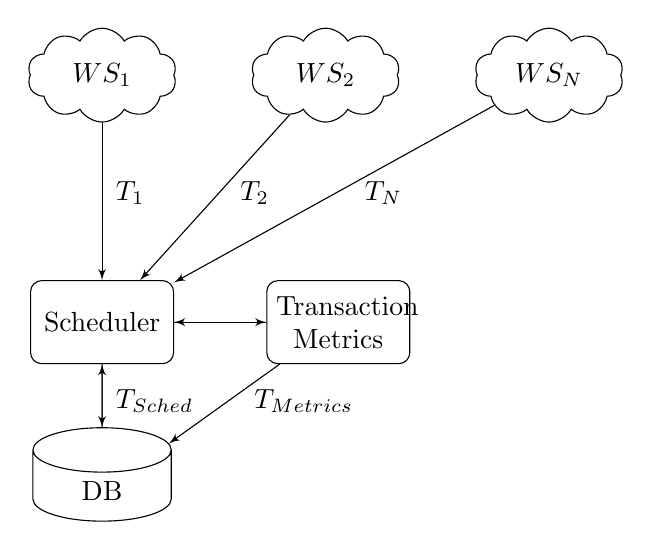
\begin{tikzpicture}
    \node [draw, cylinder, shape border rotate=90, aspect=0.75, %
      minimum height=30, minimum width=50] (data) {DB};
    \node [block, above=2cm of data.south,anchor=south] (sched) {Scheduler};
    \node [block, right=3cm of sched.south,anchor=south] (trans_met) {Transaction Metrics};
    \node [webservice, above=2cm of sched] (ws1) {$WS_{1}$};
    \node [webservice, right=of ws1] (ws2) {$WS_{2}$};
    \node [webservice, right=of ws2] (wsN) {$WS_{N}$};
    \path [line] (sched) -- (data);
    \path [line] (data) -- (sched);
    \path [line] (ws1) -- (sched);
    \path [line] (ws2) -- (sched);
    \path [line] (wsN) -- (sched);
    \path [line] (trans_met) -- (sched);
    \path [line] (sched) -- (trans_met);
    \path [line] (trans_met) -- (data);
    \put(5,105){$T_{1}$}
    \put(50,105){$T_{2}$}
    \put(95,105){$T_{N}$}
    \put(5,30){$T_{Sched}$}
    \put(55,30){$T_{Metrics}$}
\end{tikzpicture}

\caption{Web Service Environment with Transaction Metrics at Scheduling Level} % title of the Figure
\label{fig:ws_env_with_metrics} % label to refer figure in text

\end{figure}

\subsection{Categorization Graph}
\label{section_cat_graph}

% The objective bounds that the system can be measured against must be set for commit and abort rate percentages and also for the upper and lower bounds for rate of efficiency. A static value could be used for these bounds but then the solution would not be flexible for different environments. Another considered solution could store the category bounds in a relation within the local database but then this approach places the responsibility on the database administrator to ensure the bounds are appropriate for the execution environment. In order to allow the categorization bounds to flex within the execution environment while also allowing the flexibility without the aid of an administrator, we created the categorization graph.

The categorization graph is grouped into four sections where each section represents a category that a transaction can be placed. Categorization bounds (see Definition \ref{cat_bounds}) seperate the graph into four sections and determine what locking techniques the transaction will receive once placed. Transactions are graphed based on the percentages of their previous execution metrics in comparison to the other transactions executing on the same system. This allows the system to flex accordingly with different environments without the aid of an administrator. Depending on the metrics that each transaction possesses, the transactions will be categorized into the previous four categories listed above: LCLE, HCLE, HCHE, and LCHE. Transactions categorized as LCLE must have an efficiency rate that is in the 50 percentile or lower where the commit rate is also in the 50 percentile or lower (Definition \ref{ext_abrt}). Transactions categorized as HCLE must have an efficiency rate that is also in the 50 percentile or lower however the commit rate must be in the 50 percentile or higher (Definition \ref{ext_commit}). LCHE transactions must have an efficiency rate that is in the 50 percentile or higher where the commit rate is in the 50 percentile or lower (Definition \ref{min_abrt}). Transactions categorized as HCHE must have an efficiency rate that is in the 50 percentile or higher where the commit rate is also in the 50 percentile or higher (Definition \ref{min_commit}). Figure \ref{graph:cat_graph} shows the categorizations described above.


\begin{figure}[ht]
\captionsetup{justification=centering}
\centering % used for centering Figure
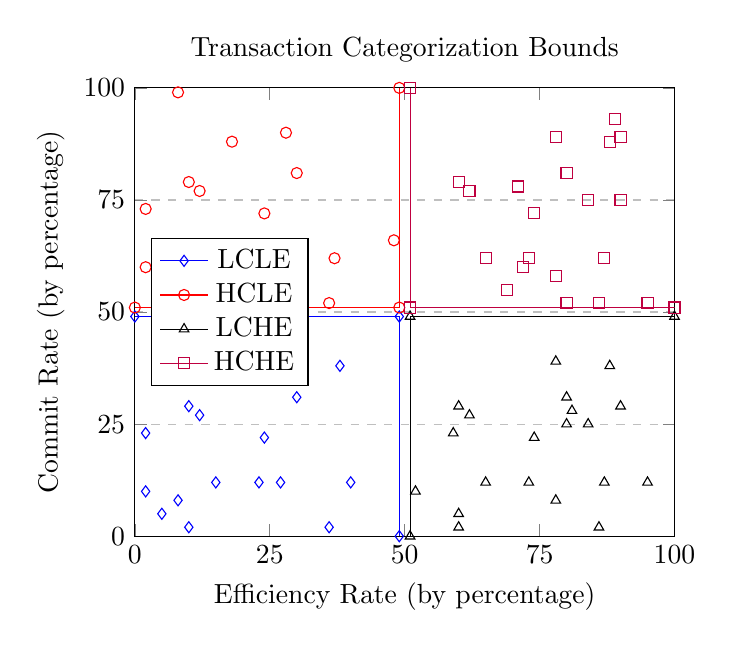
\begin{tikzpicture}
\begin{axis}[
    title={Transaction Categorization Bounds},
    xlabel={Efficiency Rate (by percentage)},
    ylabel={Commit Rate (by percentage)},
    xmin=0, xmax=100,
    ymin=0, ymax=100,
    xtick={0,25,50,75,100},
    ytick={0,25,50,75,100},
    legend style={at={(0.03,0.5)},anchor=west},
    ymajorgrids=true,
    grid style=dashed,
]

\addplot[
    color=blue,
    mark=diamond,
    ]
    coordinates {
    (0,49)(49,49)(49,0)};
\addplot[
    color=red,
    mark=o,
    ]
    coordinates {
    (0,51)(49,51)(49,100)};
\addplot[
    color=black,
    mark=triangle,
    ]
    coordinates {
    (51,0)(51,49)(100,49)};
\addplot[
    color=purple,
    mark=square,
    ]
    coordinates {
    (51,100)(51,51)(100,51)};
\addplot[
    only marks,
    color=red,
    mark=o,
    ]
    table {
    10  52
    2   60
    8   58
    5   55
    24  72
    30  81
    15  62
    10  79
    18  88
    28  90
    23  62
    12  77
    37  62
    48  66
    36  52
    8   99
    27  62
    2   73
    };
\addplot[
    only marks,
    color=blue,
    mark=diamond,
    ] 
    table {
    10  2
    2   10
    8   8
    5   5
    24  22
    30  31
    15  12
    10  29
    38  38 
    23  12
    12  27
    40  12
    36  2
    8   49
    27  12
    2   23
    };
\addplot[
    only marks,
    color=black,
    mark=triangle,
    ] 
    table {
    60  2
    52  10
    78  8
    60  5
    74  22
    80  31
    65  12
    60  29
    88  38 
    73  12
    62  27
    95  12
    86  2
    78  39
    87  12
    59  23
    80  25
    81  28
    84  25
    90  29
    };
\addplot[
    only marks,
    color=purple,
    mark=square,
    ] 
    table {
    80  52
    72  60
    78  58
    69  55
    74  72
    80  81
    65  62
    60  79
    88  88 
    73  62
    62  77
    95  52
    86  52
    78  89
    87  62
    89  93
    90  75
    71  78
    84  75
    90  89
    };

\legend{LCLE, HCLE, LCHE, HCHE}
 
\end{axis}
\end{tikzpicture}
\caption{Categorization Graph} % title of the Figure
\label{graph:cat_graph} % label to refer figure in text
\end{figure}

% \subsection{Transaction Concentration Ratio}
% \label{sec:TCR}

% As mentioned above, the categorization thresholds will flex depending on the execution environment that the transactions are a part of. This ensures that the thresholds that the categorization selection algorithm depends upon will be as accurate as possible. In order to obtain the most accurate thresholds within a changing environment we calculate the transaction concentration ratio. The transaction concentration ratio is a ratio between the sum of all transactions within a certain range on the categorization graph over the area of that range. The ratio is calculated using the formula below

% \[\textrm{$T_{Ratio}$} =\frac{\textrm{$T_{xy}{Count}$}}{x * y}\]

% In this ratio equation the $x$ represents the base length (x-axis) of the range that is taken into consideration where $y$ represents the height of the range (y-axis) that is taken into consideration. $T_{xy}{Count}$ is the sum of all transactions within the $x$ and $y$ range provided. Example \ref{ex_transaction_ratio} outlines the use of this equation.

%  \begin{example}
%  \label{ex_transaction_ratio}
%   We are calculating the concentration of transactions within the HCHE categorization zone. The base (x-axis) of the concentration zone is 20 and the height (y-axis) of the concentration zone is 15. The number of transactions that fall within this concentration range is 120. With these metrics we can form the following equation:
  
%   \[\textrm{$T_{Ratio}$} =\frac{\textrm{120}}{20 * 15}\]
%   \[\textrm{$T_{Ratio}$} =\frac{\textrm{2}}{5}\]
  
%   With these figures we can calculate that the ratio of transactions to the area of the range that the transactions were graphed is \( \frac{2}{5} \).
  
%  \end{example}
 
% Once a ratio has been calculated for each range within a categorization zone the $x$ and $y$ values of the highest ratio calculated for that zone will be used as the thresholds. In the event that there are multiple ratios calculated for a particular zone of the same value, the concentration ratio with the largest denominator in the equation will be used. By using the largest acceptable threshold we increase the number of transactions that are categorized into the categorization zone and also decrease the number of transactions that are categorized into the default NO\_TREND category\footnote{Algorithm \ref{alg:cat_for_trans} makes use of these thresholds for the selection of categories for each transaction}. This increases the number of transactions that will be executed with more appropriate locking and scheduling techniques. Example \ref{ex_transaction_ratio_2} elaborates on this situation.

%  \begin{example}
%  \label{ex_transaction_ratio_2}
%  Building from Example \ref{ex_transaction_ratio} we build a situation where the base (x-axis) is 10 and the height (y-axis) is 15. The number of transactions within this range is 60. With these metrics we form the following equation:
 
%   \[\textrm{$T_{Ratio}$} =\frac{\textrm{60}}{10 * 15}\]
%   \[\textrm{$T_{Ratio}$} =\frac{\textrm{2}}{5}\]
  
%   As shown in Example \ref{ex_transaction_ratio} we can see that the ratios are the same however this example contains half as many transactions as the previous example. By using the $x$ and $y$ thresholds in this example versus the $x$ and $y$ thresholds in Example \ref{ex_transaction_ratio}, we decrease the number of categorized transactions by 50\%.
 
%  \end{example}
 
\subsection{Category Selection}
 Concurrent transactions that are submitted to the scheduler are graphed on the Transaction Categorization Graph (see Figure \ref{graph:cat_graph}) which will therefore place the transaction into one of the four categories based on the metadata stored about the transaction. At this point serializable schedules can now be formed. The set of transactions that are submitted to the scheduler will be composed within one or many serializable schedules depending on the transactions categories. Any transaction that is contained within a conflicting category (see Definition \ref{conflict_cat}) will be the sole transaction within a serializable schedule. This is a key component of the prediction-based solution that ensures consistency among known transactions. By allowing a misbehaving transaction to execute solely without the interleaving of other transactions, this prevents cascading rollbacks and inconsistent states within the database. Any transactions that are not contained within a conflicting category will be scheduled within a separate serializable schedule that contains other transactions of non-conflicting categories. This separation of conflicting and non-conflicting transactions allows for concurrent execution of transactions but with the reduction of cascading rollbacks and the increase in consistency.

\section{Analysis}
The primary contribution of this paper provides a solution that guarantees consistency in a web service environment for concurrent transactions. In order to accomplish this contribution a combination of predictive analytics and locking with custom actions were established depending on the categorization of this transaction; therefore this solution is guaranteed to execute concurrent transactions with better or the same efficiency as traditional locking and with the consistency property intact that traditional locking provides.

\subsection{Efficiency}
We present two theorems in order to prove the improved consistency. The first theorem presented ensures that the steps taken to improve consistency do not compromise efficiency to an unacceptable state. If the efficiency of the presented solution were worse than the least efficient solution available (e.g. Traditional Locking) then the presented solution would not be of any benefit. The first theorem presented is:

\begin{theorem}
\label{theorem1}
  A serializable schedule $S_{1}$ generated from the modified scheduler in this solution will execute with an efficiency of $e_{prediction}$ where $e_{prediction} \le e_{locking}$ where $e_{locking}$ is the efficiency of the same serializable schedule $S_{1}$ executed with traditional locking techniques 
\end{theorem}

In order to prove Theorem \ref{theorem1} a proof by contradiction is used; therefore let's assume it's false and $e_{prediction} > e_{locking}$. This is the only case within the defined theorem that allows it to be proven false. 

The prediction based solution presented increases its rate of efficiency by the use of concurrent execution of well behaving transactions. This is made possible by the use of the locking techniques presented in Tables \ref{tbl:read_lock_compatibility} \& \ref{tbl:write_lock_compatibility}. The existing solution, traditional locking, ensures a serial execution of transactions within a database schedule. This solution does not allow concurrent execution of transactions and therefore suffers in efficiency. To contradict the presented theorem we must first attempt to prove that a concurrent execution of a database schedule would be less efficient than a serial execution of the same schedule.

We present two schedules: $S_{c}$, the concurrent execution of a schedule, and $S_{l}$, the serial execution of a schedule using locking techniques. Both schedules contain the same two transactions, $T_{1}$ and $T_{2}$. $T_{1}$ executes with a time of $t_{1}$ and $T_{2}$ executes with a time of $t_{2}$. The execution of a transaction always requires some amount of time to complete; therefore $t_{1} > 0$ and $t_{2} > 0$. 

\[ \textrm{$S_{c} = T_{1}T_{2}$ \textit{where} $T_{1}$ = $t_{1}$ \textit{and} $T_{2}$ = $t_{2}$} \]
\[ \textrm{$S_{l} = T_{1}T_{2}$ \textit{where} $T_{1}$ = $t_{1}$ \textit{and} $T_{2}$ = $t_{2}$} \]
\[ \textrm{\textit{where} $t_{1} > 0$ \textit{and} $t_{2} > 0$}\]

Since $S_{c}$ executes transactions $T_{1}$ and $T_{2}$ concurrently the execution time will equate to the maximum of $t_{1}$ and $t_{2}$. However, the execution time of $S_{l}$ will result in the sum of $t_{1}$ and $t_{2}$ due to the serial execution enforced by locking. We represent the total time for $S_{c}$ as $t_{total,c}$ and $S_{l}$ as $t_{total,l}$.

\[\textrm{$t_{total,c}$ = \textit{max($t_{1}$,$t_{2}$)}}\]
\[\textrm{$t_{total,l}$ = $t_{1} + t_{2}$}\]

Now that equations have been established for the total time for each schedule execution, a contradicting result can attempt to be proven by solving $t_{total,c} > t_{total,l}$.

\[\textrm{$t_{total,c} > t_{total,l}$}\]
\[\textrm{\textit{max($t_{1}$,$t_{2}$)} $> t_{1} + t_{2}$}\]

At this point in the proof there are two possible situations that affect the left side of the equation. Either $t_{1}$ or $t_{2}$ will be selected as the maximum but for completeness, both situations are accounted for.

\[\textrm{\textit{if} $t_{1} \ge t_{2}$ \textit{then} $t_{1} > t_{1} + t_{2}$}\]
\[\textrm{$0 > t_{2}$}\]
\[\textrm{\textit{if} $t_{1} < t_{2}$ \textit{then} $t_{2} > t_{1} + t_{2}$}\]
\[\textrm{$0 > t_{1}$}\]

After solving for $t_{1}$ and $t_{2}$ we see that they both are less than zero. Therefore in order for the concurrent schedule, $S_{c}$, to execute less efficiently than the serial schedule, $S_{l}$, one of the two transactions, $T_{1}$ or $T_{2}$, in $S_{l}$ must execute with a time less than zero. Since this is not possible due to the constriction stated above (e.g. $t_{1} > 0$ and $t_{2} > 0$) this proves that a successful execution of transactions concurrently will always be more efficient than a serial execution.

Now that we have established that concurrent executions are more efficient than serial executions, we can extend this proof to the locking techniques established in Table \ref{tbl:read_lock_compatibility} \& \ref{tbl:write_lock_compatibility}. Table \ref{tbl:read_lock_compatibility} displays all locking techniques within the prediction-based solution along with their associated actions if a read-lock is already granted. Table \ref{tbl:write_lock_compatibility} displays all locking techniques with their associated actions if a write-lock is already granted. After reviewing the tables it is apparent that all categories established, with the exception of LCHE transactions, contain some form of shared locking techniques. It is these categories that we can extend the previous contradiction proof and say with confidence that transactions categorized within these categories are contained within $e_{prediction} \le e_{locking}$ presented in Theorem \ref{theorem1}.

To prove the case for LCHE transactions the set theory equality proof is used on the associated lock types. Transactions contained within this category are associated with all lock types. Transactions executing with traditional locking techniques are also associated with all lock types. Therefore we can use the set equality proof to establish the equality of behavior between these two techniques based on the allowed locks. 

$L_{ma}$ represents the set of lock types available to transactions categorized as LCHE and $L_{tl}$ represents the set of lock types available to transactions using traditional locking techniques. The lock types within the sets are the lock types that are a part of the prediction-based solution in Table \ref{tbl:read_lock_compatibility}.

\[\textrm{$L_{ma} = \{S_{R},S_{W},E_{R},E_{W},I_{R},I_{W}\}$}\]
\[\textrm{$L_{tl} = \{S_{R},S_{W},E_{R},E_{W},I_{R},I_{W}\}$}\]

To prove set equality we must first show that $L_{ma} \subseteq L_{tl}$ and then show $L_{tl} \subseteq L_{ma}$. In order for $L_{ma} \subseteq L_{tl}$ we must show that for each $x$ if $x \in L_{ma}$ then $x \in L_{tl}$. By analyzing each element in $L_{tl}$ it is apparent that each element in $L_{ma}$ is contained within $L_{tl}$ and therefore $L_{ma} \subseteq L_{tl}$. Now we must show that $L_{tl} \subseteq L_{ma}$ by showing for each $x$ if $x \in L_{tl}$ then $x \in L_{ma}$. This too is true because each lock type present in $L_{tl}$ is also found in $L_{ma}$; therefore showing that $L_{tl} \subseteq L_{ma}$ and proving $L_{tl} = L_{ma}$.

In addition to $L_{tl}$ and $L_{ma}$ there are values $e_{tl}$ and $e_{ma}$ which represent the efficiency of traditional locking and LCHE transactions. $e_{tl}$ and $e_{ma}$ are directly related to the lock types assigned to their corresponding sets. The higher the value of $\left\vert{L}\right\vert$, where $L$ is a set of lock types, the lower the amount of concurrency is allowed and the lower the $e$ value. Since it is proven from the set theory of equality that $L_{tl} = L_{ma}$ it is also proven that $e_{tl} = e_{ma}$. This proves that LCHE transactions will execute with equal efficiency as traditional locking transactions and formally proves Theorem \ref{theorem1} in its entirety. 

\subsection{Consistency}
While the first theorem presented ensures the efficiency for the prediction-based solution is guaranteed to better than or equal to traditional locking, the second theorem is concerned with the consistency. The main contribution of this solution is to ensure consistency within a web service environment is equal to that of traditional locking. The second theorem presented is:

\begin{theorem}
\label{theorem2}
 $C_{prediction}$ and $C_{locking}$ are objective values obtained from running the serializable schedule $S_{1}$ with the prediction-based solution and with traditional locking. $C_{prediction}$ and $C_{locking}$ represent the consistent state of the database. $C_{prediction} = C_{locking}$ and since it is known traditional locking maintains consistency within the database then the prediction-based solution maintains consistency
\end{theorem}

The proof for this theorem will be much like Theorem \ref{theorem1} in that we will use a proof by contradiction. The proof will attempt to prove that $C_{prediction} \neq C_{locking}$ by proving a lack of consistency in the prediction-based solution. Since it is known that traditional locking ensures consistency within a database by enforcing the atomicity and isolation properties, disproving the consistency of this technique would be impossible. Instead, the proof will attempt to prove a lack of consistency in the prediction-based system by showing that a cascading rollback can occur\footnote{This proof assumes that transactions behave according to the category that they were placed in. Corollary \ref{corollary1} addresses transactions that do not behave as predicted.}.

In order to attempt to prove the lack of consistency we begin with a schedule $S_{1}$ containing two transactions, $T_{1}$ and $T_{2}$. The operations of the transactions within the schedule are interleaved and dependent upon one another. This is a key factor in order for a cascading rollback to be possible (see Definition \ref{casc_rollback}). Another key factor in order for a cascading rollback to occur is that either $T_{1}$ or $T_{2}$ must issue an abort and rollback its changes. If we assume that transactions $T_{1}$ and $T_{2}$ have the needed attributes to establish a cascading rollback within the schedule, then $T_{1}$ and $T_{2}$ also have the needed requirements to be considered conflicting transactions (see Definition \ref{conflict_trans}). Within the prediction-based solution presented, conflicting transactions are directly related to conflicting categories (see Definition \ref{conflict_cat}). This contradicts the given schedule, $S_{1}$, due to the definition of conflicting categories. The definition states that two transactions in conflicting categories, within the prediction-based solution, are not allowed within the same schedule. If conflicting categories are not allowed within the same schedule then we can also assume with confidence that conflicting transactions will not ever be present together within the same schedule. Therefore, with conflicting transactions always in separate schedules we can prove that no cascading abort will occur in the prediction-based solution. This ensures that consistency is always kept within the system and contradicts that $C_{prediction} \neq C_{locking}$ and thus proves Theorem \ref{theorem2} by proving $C_{prediction} = C_{locking}$.

\subsection{Unpredictable Aborts}
The prediction-based solution presented can handle transactions that both commit and abort while maintaining consistency but issues arise when transactions that have been predicted correctly execute with unpredictable results. If we have serializable schedule $S_{1}$ which contains \textit{n} number of interleaved non-conflicting transactions but transaction $T_{i}$ issues an unexpected and unpredictable abort the system must be able to regain consistency. The obtainment of consistency must perform better than or equal to a typical web service environment in order for the prediction-based solution to be feasible. With that very thought in mind we present the following corollary to the previous two theorems:

\begin{corollary}
\label{corollary1}
 In the event that a serializable schedule $S_{1}$ generated from the modified scheduler in this solution compromises the consistency of the database it must re-establish consistency in $t_{prediction}$ where $t_{prediction} \le t_{web service}$ where $t_{web service}$ is the time cost to re-establish consistency in existing web service environments and $t_{prediction}$ is the time cost to re-establish consistency in the prediction-based solution presented
\end{corollary}

Much like the previous two proofs, a proof by contradiction is used to establish that $t_{prediction} \le t_{web service}$. The proof will attempt to prove that $t_{prediction} > t_{web service}$ since this is the only case that will contradict the given corollary. We begin by establishing two schedules; $S_{p}$, a schedule executed by the prediction-based system and $S_{ws}$, a schedule executed within a typical web service environment. Both schedules are identical and are composed of transactions $T_{1}$ and $T_{2}$. The operations of the two transactions are interleaved and dependant upon one another; therefore requiring a cascading rollback to restore consistency in the event of an unexpected abort.

\[\textrm{$S_{p} = T_{1}T_{2}$}\]
\[\textrm{$S_{ws} = T_{1}T_{2}$}\]

During the execution of both schedules an abort is issued and two transactions are generated: $T_{gen,p}$ and $T_{gen,ws}$. $T_{gen,p}$ is a generated transaction from the modified scheduler to reestablish consistency within the database. $T_{gen,ws}$ is also a generated transaction from the typical web service environment scheduler to reestablish consistency. Although, the scheduler in the prediction-based solution is modified to add needed functionality, the functionality to generate compensation transactions is the existing functionality contained in both schedulers. By using the same generation process to generate compensation transactions $T_{gen,p}$ and $T_{gen,ws}$ on schedules $S_{p}$ and $S_{ws}$ with the same transactions, we can then say with confidence that $T_{gen,p} = T_{gen,ws}$. With $T_{gen,p} = T_{gen,ws}$ it is contradicting to state that $t_{prediction} > t_{web service}$ when the process is in fact equal. Therefore we conclude that $t_{prediction} = t_{web service}$ and formally prove Corollary \ref{corollary1}.

\begin{algorithm}
\caption{Top Level Scheduler Algorithm}
\label{alg:top_level}
\begin{algorithmic}[1]

\Procedure{manage\_transactions}{}
  \State // This method is the top level procedure call
  \State // that will be called as long as transactions
  \State // are available and need to be scheduled
  \State // for execution
  \\
  \State Transaction[] trans;
  \While{true}
    \State // Clears the list from last execution
    \State trans.\Call{clear}{}
    \\
    \State // This method gets the available transactions that
    \State // are submitted to the scheduler for processing.
    \State // This includes preemptively aborted transactions
    \State // from previous executions
    \State Transaction[] aborted = \Call{getAbortedTrans}{}
    \State Transaction[] schedTrans = \Call{getSchedTrans}{};
    \\
    \State // Adds the available transactions from the
    \State // scheduler to the overall collection of
    \State // transactions that need to be scheduled. 
    \State // These are added behind any transactions that
    \State // were aborted from the previous execution
    \State trans.\Call{add}{aborted};
    \State trans.\Call{add}{schedTrans};
    \\
    \State // Generates serializable schedules from the 
    \State // available transactions
    \State SerialSched[] ss = \Call{generate\_schedules}{trans};
    \\
    \State // Orders the generated schedules according to their
    \State // priorities
    \State ss = \Call{order\_schedules}{ss};
    \\
    \State // Executes each generated schedule. Transactions
    \State // that are aborted preemptively will be scheduled
    \State // in the next execution
    \ForAll{s in ss}
      \State \Call{exec\_sched}{s};
    \EndFor
  \EndWhile
\EndProcedure

\end{algorithmic}
\end{algorithm}

\section{Algorithms}
\label{sec:algorithms}
In the existing web service environment the scheduler is the first stage of the system where the transactions are submitted for processing. At this point, serializable schedules are created from the concurrent transactions and executed on the database for processing. The transaction metrics solution begins here with Algorithm \ref{alg:top_level}. The algorithm implemented in Algorithm \ref{alg:top_level} is a simulation of how schedulers execute continuously and obtain transactions to be submitted for processing. The function call within the scheduler may not be known but, for purposes of explanation, it is called \textit{manage\_transactions}. The first step in this algorithm is to gather any aborted transactions from the previous execution and any new incoming transactions. Once this step is complete, the scheduler initiates the process and continues to Algorithm \ref{alg:generate_sched}. This algorithm generates the serializable schedules based on the proposed solutions parameters.This algorithm will be further analyzed later in this section. After the serializable schedules have been generated from the given transactions they must be ordered appropriately from the priorities given above. At this point, Algorithm \ref{alg:priority_algorithm} will be executed. This algorithm will also be discussed in further detail later in this section. Once the correct ordering of the serializable schedules have been determined, each schedule will be executed using Algorithm \ref{alg:exec_sched}. This uses the existing logic of the DBMS along with other custom logic in order to perform the execution. Along with the execution, it also updates the transaction metrics appropriately in order to build a more accurate prediction. Each execution of Algorithm \ref{alg:exec_sched} is within an independent thread to prevent a bottleneck in the process. An asynchronous procedure call back to the scheduler will send any aborted transactions that were preemptively aborted and need to be rescheduled. This algorithm will also be discussed in detail to elaborate on the updating of Transaction Metrics. Once this algorithm has completed, the top-level scheduling algorithm, returns to the top of its processing loop and repeats the same process. The next sections give an explanation of the algorithms mentioned above that compose this entire process.

\begin{algorithm}
\caption{DBMS Scheduler Generation Algorithm}
\label{alg:generate_sched}
\begin{algorithmic}[1]

 \Function{generate\_schedules}{Transaction[] trans} 
   \\
   \State // Create map of transaction and category
   \State // relationships
   \State Map[Transaction, Category] transCats;
   \ForAll{t in trans}
      \State // Transaction Metrics Algorithm Function Call
      \State // Function call will take a max of O(1) time
      \State // to complete.
      \State Category c = \Call{getCatForTrans}{t}; \label{l:getcatfortrans}
      \\
      \State // Assign lock behavior to the transaction from
      \State // the compatibility matrices provided. The 
      \State // lock behaviors are associated directly with
      \State // a category
      \State LockBehavior[] lb = c.\Call{getLockBehaviors}{}; 
      \State t.\Call{setLockBehaviors}{lb}; \label{l:setlockbehaviors}
      \\
      \State transCats.\Call{add}{t,c}; \label{l:tcadd}
   \EndFor
   \\
   \State // Create collection of serializable schedules to
   \State // be returned
   \State SerialSched[] schedules;
   \State // Create temporary collection of non-conflicting
   \State // transactions
   \State Transaction[] nonConflictingTrans;
   \ForAll{entry in transCats}
      \State // Method call to determine if the category 
      \State // passed in will conflict with other transactions
      \State // based on the definition of conflicting transactions
      \State bool isConflict = \Call{isCatConflict}{entry.cat};
      \If{isConflict}
        \State // Generate serializable schedule with only one
        \State // transaction using the existing scheduler 
        \State // mechanism
        \State SerialSched s = \Call{genSchedule}{entry.trans};\label{l:gencsched}
        \State schedules.\Call{add}{s};
      \Else
        \State // Add transaction to a temporary collection
        \State // to generate schedule
        \State nonConflictingTrans.\Call{add}{entry.trans}; \label{l:tempds}
      \EndIf
   \EndFor
   \\
   \State // Generate a bulk schedule composed of 
   \State // non-conflicting transactions that can execute
   \State // concurrently without consequence
   \State SerialSched s = \Call{genSchedule}{nonConflictingTrans};\label{l:bulksched}
   \State schedules.\Call{add}{s};
   \\
   \State \Return schedules; \label{l:rtnsched}
 \EndFunction
 
\end{algorithmic}
\end{algorithm}

\subsection{Generate Schedules}
The process of generating schedules from incoming transactions will use the existing logic in the scheduler however this functionality is overloaded. The overloaded logic of generating schedules includes two additional actions: 1.) assigning the correct lock behaviors provided by Tables \ref{tbl:read_lock_compatibility} \& \ref{tbl:write_lock_compatibility} and 2.) generating separate schedules based on conflicting and non-conflicting transactions derived from the definition of conflicting transactions (see Definition \ref{conflict_trans}). The first part of the algorithm steps through each transaction passed in as an argument and obtains the category for that particular transaction by the execution of Algorithm \ref{alg:cat_for_trans} (line.\ref{l:getcatfortrans}); which will be discussed in a later section. After the categorization of the transaction has been obtained, the correct lock behaviors that are allowed by categorization (referenced in Tables \ref{tbl:read_lock_compatibility} \& \ref{tbl:write_lock_compatibility}) are enforced on the particular transaction (line.\ref{l:setlockbehaviors}) and both the transaction and the category are placed in a temporary data structure in order to store the relationships (line.\ref{l:tcadd}). The second part of the algorithm generates the schedules based on conflicting and non-conflicting transactions. By generating dedicated schedules for transactions that are predicted to conflict with others, this prevents conflicting transactions from causing a cascading rollback on a serializable schedule with transactions that are sure to execute successfully. In this part of the algorithm a dedicated serializable schedule is created for any transaction that is considered conflicting (line.\ref{l:gencsched}) while transactions that are not considered conflicting are stored in a temporary data structure (line.\ref{l:tempds}). Once all transactions have been analyzed, all transactions that are not considered conflicting in the temporary data structure are composed into a single interleaved serializable schedule for the database to execute (line.\ref{l:bulksched}). Since we know the transactions will commit the outcome to the database we can allow these transactions to execute concurrently with confidence that a cascading rollback will not be required. After all serializable schedules have been generated the algorithm returns the collection of schedules (line.\ref{l:rtnsched}).

\begin{algorithm}
\caption{T.M. Category Determination Algorithm}
\label{alg:cat_for_trans}
\begin{algorithmic}[1]

 \Function{getcatfortrans}{Transaction t}
    \\
    \State // Category enum to be returned
    \State Category c;
    \\
    \State // Obtain ID from transaction
    \State String id = t.id; \label{l:tid}
    \\
    \State // Execute query to obtain transaction information
    \State // This transaction does not have to worry about
    \State // concurrency control issues since it is only
    \State // known to this logical unit
    \State MetricsData data = \Call{getMetricsData}{id};\label{l:metdata}
    \\
    \State // Categorization Graph data is also stored 
    \State // in the database so that the categorization 
    \State // bounds can be used easily. This data must 
    \State // be returned before evaluation
    \State TransBounds bounds = \Call{getTransBounds}{};\label{l:boundsdata}
    \\
    \State // Evaluate the data returned and return the category
    \If{data.ER\_rate $>=$ bounds.ER\_rate} \label{l:start_eval}
        \If{data.exec\_t $>=$ bounds.exec\_t}
           \State c = HCLE;
         \Else
           \State c = HCHE;
         \EndIf
    \Else
         \If{data.exec\_t $>=$ bounds.exec\_t}
           \State c = LCLE;
         \Else
           \State c = LCHE;
         \EndIf
    \EndIf \label{l:end_eval}
    \\
    \State \Return c;
 \EndFunction

\end{algorithmic}
\end{algorithm}

\subsection{Get Category For Transaction}
As a part of the \textit{generate schedule} algorithm mentioned above, a helper function was required in order to obtain the category based on a particular transaction. This helper function is outlined in Algorithm \ref{alg:cat_for_trans}. The first part of the algorithm obtains the unique identifier used to identify a transaction among other transactions submitted for processing (line.\ref{l:tid}). Once an identifier is obtained, the Transaction Metrics data is obtained by the identifier provided (line.\ref{l:metdata}) and the categorization thresholds set by the Categorization Graph for commit rate and efficiency rate (line.\ref{l:boundsdata})\footnote{This data is pulled by a SQL query from the database that can use traditional locking techniques since the relations storing this data are only known to the scheduler and Transaction Metrics units}. Once this data is available the appropriate evaluations are made to ensure that the correct category is chosen for the transaction provided (lines.\ref{l:start_eval}-\ref{l:end_eval}). The evaluations made are based on the data presented in Table \ref{tbl:default_tmetrics}. After a category has been evaluated, an enumeration is set with the correct category and returned.

% \begin{algorithm}
% \caption{Calculate Categorization Threshold}
% \label{alg:calc_threshold}
% \begin{algorithmic}[1]

%  \Procedure{calcCategoryThresholds}{}
%   \ForAll{c in CATEGORIES} \label{l:each_cat}
%     \State real $ratio$ = 0.0;
%     \State int $p_x$, $p_y$, $s_x$, $s_y$, $e_x$, $e_y$;
%     \State $s_x$ = \Call{getstartval}{x,c}; \label{l:getstart}
%     \State $s_y$ = \Call{getstartval}{y,c};
%     \State $e_x$ = \Call{getendval}{x,c};
%     \State $e_y$ = \Call{getendval}{y,c}; \label{l:getend}
%     \\
%     \ForAll{x between $s_x$ and $e_x$} \label{l:forx}
%       \ForAll{y between $s_y$ and $e_y$} \label{l:fory}
%         \State real $tmpRatio$;
%         \State int $c_x$, $c_y$, $t_{count}$;
%         \State $c_x$ = $|x$ - $s_x|$; \label{l:absx}
%         \State $c_y$ = $|y$ - $s_y|$; \label{l:absy}
%         \State $t_{count}$ = \Call{getNumOfTrans}{$c_x$,$c_y$}; \label{l:numtcount}
%         \\
%         \State $tmpRatio$ = $\dfrac{t_{count}}{c_x * c_y}$ \label{l:tmpratio}
%         \\
%         \If{$ratio > tmpRatio$} \label{l:comparestart}
%         \State // Already have a larger ratio.
%         \State // Do nothing
%         \ElsIf{$ratio < tmpRatio$}
%         \State // New ratio is larger than previous so
%         \State // we update our current values
%         \State $ratio = tmpRatio$; \label{l:ratiohigher_start}
%         \State $p_x = c_x$;
%         \State $p_y = c_y$;\label{l:ratiohigher_end}
%         \Else \label{l:equalstart}
%         \State // The ratio is equal so we must
%         \State // determine the greatest denominator
%         \State // and choose that one
%         \If{$(p_x * p_y) \ge (c_x * c_y)$}
%         \State // Values already set so we can just
%         \State // do nothing
%         \Else
%         \State $p_x = c_x$;
%         \State $p_y = c_y$;
%         \EndIf
%         \EndIf \label{l:compareend}
%       \EndFor
%     \EndFor
%     \\
%     \State // Once the largest threshold values are 
%     \State // obtained we can write them to disk
%     \State // for the categorization selection 
%     \State // algorithm to use
%     \State \Call{writetodb}{$p_x, p_y, c$}; \label{l:writetodb}
%     \State $p_x, p_y, ratio = 0$; \label{l:reset}
%   \EndFor
%  \EndProcedure

% \end{algorithmic}
% \end{algorithm}

% \subsection{Calculate Categorization Thresholds}
% Calculating the categorization thresholds for each category is a key algorithm to the solution in that it ensures the most accurate thresholds for which transactions will be categorized. This algorithm is executed after each transaction is submitted to the database. Due to the complexity of this algorithm a multi-threaded approach was taken to ensure that the selection of categories for each transaction would not contain the overhead of wait time.

% The first step of this algorithm is to step through each category available (line.\ref{l:each_cat}). This does not include the NO\_TREND category since this is the default category that transactions are placed if a categorization cannot be made. For each category that needs calculated thresholds we obtain the start and end values for both the x and y axis (lines.\ref{l:getstart}-\ref{l:getend}). This is a key section of the algorithm to ensure the correct calculations are made. For example, if the LCLE category was processed the start values for both axes would be 0 and the end values would be 25. However for a HCHE transaction the start values for both axes would be 100 and the end values would be 75. Once the start and end values are obtained we step through each possible x-value and y-value within each range (lines.\ref{l:forx} and \ref{l:fory}). For every x and y-value within the ranges, we calculate the absolute value of the current value subtracted from the start value (lines.\ref{l:absx} and \ref{l:absy}). In some cases the current value will always be greater than the start value (e.g. LCLE) but in other cases it will not (e.g. HCHE). By using the absolute value we are always guaranteed to have the positive x and y-values from which we are going to calculate the ratio. Next we count the number of transactions within the particular range (line.\ref{l:numtcount}). Once the transaction count is obtained we calculate a ratio of the number of transactions divided by the area of the particular range (line.\ref{l:tmpratio}). Once that ratio is calculated we compare it to highest ratio that was calculated for this particular category. At this point it becomes a simple comparison between which is higher and lower (lines.\ref{l:comparestart}-\ref{l:compareend}). If the new ratio is higher, it is cached and the new thresholds are also cached (lines.\ref{l:ratiohigher_start}-\ref{l:ratiohigher_end}). If the new ratio is lower, the algorithm continues processing (line.\ref{l:comparestart}). In the event that the new ratio is equal to the highest ratio for that category, the largest denominator will be stored (lines.\ref{l:equalstart}-\ref{l:compareend}). Once the thresholds have been calculated for each comparison for that particular category, the thresholds will be sent to the local relation through an SQL query (line. \ref{l:writetodb}). This will ensure that when Algorithm \ref{alg:cat_for_trans} executes a read on the local database to obtain the most recent thresholds that they will always be up to date. This also prevents Algorithm \ref{alg:cat_for_trans} from causing a bottleneck in the performance of the system. Before processing the next category, the variables used to store the ratio and the category thresholds are reset before the next category in the collection is calculated (line.\ref{l:reset}).


\begin{algorithm}
\caption{Priority Ordering Algorithm}
\label{alg:priority_algorithm}
\begin{algorithmic}[1]

  \Function{order\_schedules}{SerialSched[] ss}
    \State // Create collection to hold the relationship
    \State // between a serializable schedule and its
    \State // priority averaged across all transactions
    \State // that compose that schedule
    \State Map[SerialSched, Integer] ssAvg; \label{l:mapstart}
    \\
    \ForAll{s in ss}\label{l:forstart}
      \State Transaction[] t = s.\Call{getTransactions}{}; \label{l:gettrans}
      \State int i = \Call{AVG}{t}; \label{l:avgt}
      \State ssAvg.\Call{add}{s,i}; \label{l:mapadd}
    \EndFor
    \\
    \State // Sort the temporary map by the priority
    \State // average
    \State \Call{sort}{ssAvg.valueSet};
    \\
    \State \Return ssAvg.keySet; \label{l:returnkeys}
    \\
  \EndFunction

\end{algorithmic}
\end{algorithm}

\subsection{Order Schedules}
Once the schedules have been generated they must be ordered by their respective priority (placed on them in Table \ref{tbl:priority}). Algorithm \ref{alg:priority_algorithm} is the function call responsible for the prioritization. In this function a data structure of serializable schedules are passed in and an ordered collection of the same schedules is returned. Before starting the ordering process, a temporary data structure is created in order to store the relationship of a serializable schedule to its priority value (line.\ref{l:mapstart}). Once the data structure is established, the algorithm steps through each serializable schedule passed in as an argument (line.\ref{l:forstart}). Within the loop, all the transactions for a particular serializable schedule are obtained and averaged (lines.\ref{l:gettrans} and \ref{l:avgt}). The average is derived from the priorities of each transaction in the serializable schedule. These priorities are related to the particular category that a transaction is categorized (see Table \ref{tbl:priority}). Once the average has been computed, the serializable schedule and the priority average associated with that schedule is placed in the temporary data structure to store the relationship (line.\ref{l:mapadd}). After all averages have been calculated for each serializable schedule that was passed in as an argument, the temporary data structure is sorted based on the value set of each relationship. The value set of the data structure is the averaged priority. Once the data structure is sorted, the key set is returned (line.\ref{l:returnkeys}). At this point the key set will be a collection of the same serializable schedules but sorted in the correct order for execution. This ensures that the collection returned is a sorted data structure with the non-conflicting serializable schedules available for execution first and the conflicting schedules last.

\begin{algorithm}
\caption{DBMS Execute Schedule Algorithm}
\label{alg:exec_sched}
\begin{algorithmic}[1]

\Procedure{exec\_sched}{SerialSched s}
    \State Transaction [] aborted;
    \State RCDS rcds = RCDS.\Call{getinstance}{}
    \\
    \ForAll{o in s}
        \State Action a;
        \If{o = WRITE}
            \State Category c = rcds.\Call{getmaxcat}{o.resrc}
            \State a = CM.\Call{getAction}{c, o.resrc}
        \Else
            \State a = CM.\Call{getAction}{o.cat, o.resrc}
        \EndIf
        \\
        \If{a = DECLINE}
            \State \Call{wait}{}
            \\
            \If{o = READ}
                \State rcds.\Call{add}{o.resrc, o.cat}
            \EndIf
            \State DBMS.\Call{submit}{o}
        \ElsIf{a = ELEVATE}
            \ForAll{l in o.resource.locks}
                \State DBMS.\Call{abort}{l.transaction}
                \State aborted.\Call{add}{l.transaction}
            \EndFor
            \\
            \If{o = READ}
                \State rcds.\Call{add}{o.resrc, o.cat}
            \EndIf
            \State DBMS.\Call{submit}{o}
        \Else
        \State rcds.\Call{add}{o.resrc, o.cat}
        \State DBMS.\Call{submit}{o}
        \EndIf
        \\
        \If{o = READ}
            \State rcds.\Call{remove}{o.resrc, o.cat}
        \EndIf
    \EndFor
    \\
    \State data = DBMS.\Call{get\_trans\_data}{}
    \ForAll{e in data}
        \State \Call{updateTMetricsData}{e.result, e.time, e.t\_id};\label{l:updatetmetrics}
    \EndFor
    \\
    \State SCHEDULER.\Call{schedule}{aborted}
\EndProcedure

\end{algorithmic}
\end{algorithm}

\subsection{Execute Schedules}
The final procedure needed in the scheduler for executing transactions is the actual execution of the generated serializable schedule. Each execution of this procedure is executed in a dedicated thread in order to prevent blocking execution in the calling scope. This is what designates the need for the Resource Category Data Structure (RCDS) (Section \ref{RCDS}). Although there may be single scheduler organizing and submitting transactions, there can be multiple concurrent executions going on with varying execution times. The RCDS keeps track of the multiple read-locks that are granted for a resource so the correct comparison can be made between executions. This function is outlined in Algorithm \ref{alg:exec_sched}.

The existing logic for executing an operation on the database within the DBMS is needed but, before the operation can be performed there are numerous conditions that have to be taken into consideration. This procedure begins by iterating through each operation contained within a serializable schedule. Before any processing can take place, the action must be obtained based on the operation's category (derived by the category placed on the transaction containing the operation) and the operated resource (Based on Tables \ref{tbl:read_lock_compatibility} \& \ref{tbl:write_lock_compatibility} and Definitions \ref{grant_action}, \ref{decline_action}, and \ref{elevate_action}). If the operation is a write, then we consult the RCDS for the highest category lock granted for the operation's resource. This is performed for only write operations because there could be different actions for different categories of requesting write locks.

If the action obtained is a \textit{decline action} then, by definition, the operation would wait until the all locks were released and then it would perform the operation. If the action obtained is an \textit{elevate action} then all current locks granted for the operations resource would be dropped, their corresponding transactions would be aborted, and then the operation would be submitted for processing. Only preemptively aborted transactions in this case are obtained and automatically resubmitted for processing. The final action, \textit{grant action} is simply submitted to the DBMS for processing. In each of the three action cases, if the operation requesting a lock is a read operation then an entry in the RCDS is added. This ensure that other executions that are occurring concurrently obtain the most accurate information for comparisons within the compatibility matrices. After the operation has completed processing from the DBMS, the entry in the RCDS is removed if it was a read operation.

After all operations have completed processing, the transactional metadata for all operation executions is retained from the DBMS. This information is then used to populate the Transactional Metrics logical unit. This step ensures that the data pulled for Algorithm \ref{alg:cat_for_trans} is always up to date and the correct categorization is always used.

The final step in the execution process is to reschedule any transactions that were preemptively aborted due to the \textit{elevate action}. These transactions are entered back into the beginning of the process by an asynchronous call back to the scheduler. This prevents any starvation that could potentially occur from preemptive transactional aborts.

\subsection{Complexity Analysis}
For each of the algorithms listed above a complexity analysis is provided for clarity and transparency. All complexity analyses are presented using Big O notation for an upper bound of the algorithm's worst case scenario.

\subsubsection{Algorithm \ref{alg:top_level}: Top Level Scheduler Algorithm}
This algorithm is used to emulate the database scheduler which will continuously obtain transactions needed for scheduling. It contains a \verb|while true| that does not provide a way for any user input to exit the infinite loop. Since there is no way to exit the execution of the scheduler, then the complexity is $O(\infty)$. However, we can analyze the inner functionality contained within the \verb|while true|.

The more important analysis for this algorithm is the time complexity before more transactions are scheduled and executed. If we analyze the complexity of the operations within the infinite loop we see a total of six operations however only three contribute to the time complexity\footnote{The fourth operation within the loop is executed within a dedicated thread to prevent any unneeded blocking.}. The first two function calls, \verb|GETABORTEDTRANS| and \verb|GETSCHEDTRANS|, are simple lookup operations responsible for getting the current transactions needed for scheduling. This executes in constant time (e.g. $O(1)$) and does not affect the total complexity. The second function call, \verb|GENERATE_SCHEDULES|, (see Section \ref{alg_complex:gen_sched}) executes with a complexity of $O(n)$. The third function call, \verb|ORDER_SCHEDULES|, (see Section \ref{alg_complexity:order_alg}) executes with a complexity of $O(n\log n)$. The final operation that impacts the overall complexity within the loop is a nested \verb|for| loop. This loop iterates over $n$ elements where $n$ is equal to the number of serializable schedules generated. The operation within this loop, the procedure call \verb|EXECUTE_SCHED| (see Section\ref{alg_complexity:exec_sched}), executes within a dedicated thread for each execution to allow concurrency of transactions. Therefore if there are $n$ schedules needing execution and each execution executes with a complexity of $O(1)$, the total complexity of the final \verb|for| is $O(n)$. With all components analyzed we see that out of the three major contributing functions that $O(n\log n)$ consumes the other two complexities and we can conclude that the total complexity within the infinite execution is an asymptotic upper bound of $O(n\log n)$.

\subsubsection{Algorithm \ref{alg:generate_sched}: DBMS Scheduler Generation Algorithm}
\label{alg_complex:gen_sched}
The \verb|GENERATE_SCHEDULES| algorithm uses the existing logic of the scheduler along with categorization data from the prediction-based solution to generate serializable schedules. There are two non-nested iterations of $n$ items where the operations in each iteration are constant. This brings the total complexity analysis of the entire algorithm to $O(2n)$ which inherently translates to an asymptotic upper bound of $O(n)$.

\subsubsection{Algorithm \ref{alg:cat_for_trans}: T.M. Category Determination Algorithm}
In this algorithm lies the responsibility of determining the category in which a transaction is placed depending on its metrics. This algorithm is designed to specifically execute in constant time so that a bottleneck is not created. A bottleneck would cause a huge performance degradation in the prediction-based solution. There are only \verb|if| comparisons within the processing logic and no \verb|for| or \verb|while| loops causing $n$ number of comparisons. Therefore, the overall complexity for the entire function is an an asymptotic upper bound of $O(1)$. 

% \subsubsection{Algorithm \ref{alg:calc_threshold}: Calculate Categorization Threshold}
% Out of all the algorithms presented in this solution, this algorithm contains most computational expensive operations. The entire algorithm is contained within a \verb|for| loop iterating through each category available. Nested within this loop is another \verb|for| loop iterating through every x-value that could be possible for that particular category (see Figure \ref{graph:cat_graph}). Within this nested loop is yet another \verb|for| loop iterating through every possible y-value for that category. At this point, every operation within the last nested loop executes in constant time and is not a factor. At this point with the three nested loops we have a complexity of $O(n^{3})$. Even though this algorithm will execute within its own dedicated thread to prevent any blocking of calling functions, this not ideal. Taking the analysis a step further we see that the first \verb|for| loop iterates through all possible categories. This is a finite number with a max of 4\footnote{There is no need to calculate thresholds for the NO\_TREND category since it will be the default case; therefore only 4 out of the 5 total categories need thresholds calculated}. The second and third \verb|for| loops are also constrained to finite number of 25 due to the categorization bounds placed on categories (see Definition \ref{cat_bounds}). With these finite bounds taken into consideration we see that the complexity is much more efficient with an upper bound of $O(4*25*25) = O(2500)$. This translates to an asymptotic upper bound of $O(1)$ or $\Theta(1)$ since we know this is a tight bound.

\subsubsection{Algorithm \ref{alg:priority_algorithm}: Priority Ordering Algorithm}
\label{alg_complexity:order_alg}
The \verb|ORDER_SCHEDULES| function orders a collection argument of serializable schedules by averaging the priorities across all transactions within that schedule. Once an average priority has been obtained for each schedule, the schedules are sorted by their average priority in ascending order. Within this algorithm, there is a single \verb|for| loop that iterates over $n$ elements. After this iteration, a collection of $n$ elements is sorted using the language's built-in sorting function. If we assume this is an optimized language we can assume the sorting will have an asymptotic tight bound of $\Theta(n\log n)$. By adding the two complex operations of the function we have a time complexity of $O(2n\log n)$ which translates to an asymptotic upper bound of $O(n\log n)$.

\subsubsection{Algorithm \ref{alg:exec_sched}: DBMS Execute Schedule Algorithm}
\label{alg_complexity:exec_sched}
The final algorithm in the analysis is the overridden \verb|EXECUTE_SCHED| procedure. This algorithm makes use of the existing logic within the DBMS to execute operations from the generated schedules. The additional logic contains an overarching \verb|for| that steps through each operation within the schedule provided to execute. There are no nested iterations within the overarching \verb|for| which equates to $O(n)$ complexity in operations. Outside of the \verb|for| there is an additional iteration for each data item recorded from the previous executions. These data items do not equate to the $n$ operations mention above so the complexity of the final iteration is $O(m)$. With these two complexities combined the final complexity analysis is $O(m+n)$ which translates to an asymptotic upper bound of $O(n)$. Although the complexity is linear, any calling components will see the execution behave in constant time. This is due to each execution of \verb|EXECUTE_SCHED| executing within its own dedicated thread to prevent any blocking on upper level function calls.

\section{Future Research}
The prediction-based Transaction Metrics solution is a flexible implementation that can be used to categorize transactions based on any criteria that a user specifies. Based on these categorizations certain steps can be taken to treat transactions differently. One area that this solution could be used is in the effort to prevent malicious transactions from corrupting the database. Malicious transactions carry certain attributes with them that can be leveraged using this solution so that they are handled differently to prevent the database from being completely useless after an execution. Liu and Jajodia implemented a multi-phase confinement system that provided a certain level of intrusion tolerance for database systems \cite{Liu_Intrusion}. We believe their model can be expanded using the Transaction Metrics in this solution. Just as the Transaction Metrics solution ensures consistency for web service transactions by prediction, we believe a molded version of the Transaction Metrics will be able to determine malicious transactions efficiently, handle them appropriately, and prevent any unwanted corruption to the database.

% if have a single appendix:
%\appendix[Proof of the Zonklar Equations]
% or
%\appendix  % for no appendix heading
% do not use \section anymore after \appendix, only \section*
% is possibly needed

% use appendices with more than one appendix
% then use \section to start each appendix
% you must declare a \section before using any
% \subsection or using \label (\appendices by itself
% starts a section numbered zero.)
%


%\appendices
%\section{Proof of the First Zonklar Equation}
%\blindtext

\section*{Conclusion}
In conclusion, transactional correctness and consistency in web service based database transactions are still an after-thought. With the compensation transactions solution, having transactions generate inconsistent states has become acceptable. The prediction-based performance metric that is proposed here is a scalable and efficient solution to web service transactions. This would drastically minimize the amount of compensation transactions needed to ensure consistency in concurrent database transactions. The solution also ensures a consistent state for transactions that have built a reputation for being reliable under the calculated performance metric.

% use section* for acknowledgement
\section*{Acknowledgment}
Special thanks to the University of South Carolina, in particular Dr. Csilla Farkas for her continued support as my research adviser. Additional thanks to The Citadel and the Department of Math and Computer Science for their support, in particular Dr. Shankar Banik for his support as my research adviser.


% Can use something like this to put references on a page
% by themselves when using endfloat and the captionsoff option.
\ifCLASSOPTIONcaptionsoff
  \newpage
\fi



% trigger a \newpage just before the given reference
% number - used to balance the columns on the last page
% adjust value as needed - may need to be readjusted if
% the document is modified later
%\IEEEtriggeratref{8}
% The "triggered" command can be changed if desired:
%\IEEEtriggercmd{\enlargethispage{-5in}}

% references section

% can use a bibliography generated by BibTeX as a .bbl file
% BibTeX documentation can be easily obtained at:
% http://www.ctan.org/tex-archive/biblio/bibtex/contrib/doc/
% The IEEEtran BibTeX style support page is at:
% http://www.michaelshell.org/tex/ieeetran/bibtex/
%\bibliographystyle{IEEEtran}
% argument is your BibTeX string definitions and bibliography database(s)
%\bibliography{IEEEabrv,../bib/paper}
%
% <OR> manually copy in the resultant .bbl file
% set second argument of \begin to the number of references
% (used to reserve space for the reference number labels box)
%\begin{thebibliography}{1}
\bibliographystyle{IEEEtran}
\bibliography{sources}
%\end{thebibliography}

% biography section
% 
% If you have an EPS/PDF photo (graphicx package needed) extra braces are
% needed around the contents of the optional argument to biography to prevent
% the LaTeX parser from getting confused when it sees the complicated
% \includegraphics command within an optional argument. (You could create
% your own custom macro containing the \includegraphics command to make things
% simpler here.)
%\begin{biography}[{\includegraphics[width=1in,height=1.25in,clip,keepaspectratio]{mshell}}]{Michael Shell}
% or if you just want to reserve a space for a photo:

%\begin{IEEEbiography}[{\includegraphics[width=1in,height=1.25in,clip,keepaspectratio]{picture}}]{John Doe}
%\blindtext
%\end{IEEEbiography}

% You can push biographies down or up by placing
% a \vfill before or after them. The appropriate
% use of \vfill depends on what kind of text is
% on the last page and whether or not the columns
% are being equalized.

%\vfill

% Can be used to pull up biographies so that the bottom of the last one
% is flush with the other column.
%\enlargethispage{-5in}




% that's all folks
\end{document}